\documentclass[12pt, twoside, openright]{report} % Fuente a 12pt, formato doble página y chapter a la derecha
\raggedbottom % No ajustar el contenido con un salto de página

% MÁRGENES: 2,5 cm sup. e inf.; 3 cm izdo. y dcho.
\usepackage[
a4paper,
vmargin=2.5cm,
hmargin=3cm
]{geometry}

% INTERLINEADO: Estrecho (6 ptos./interlineado 1,15) o Moderado (6 ptos./interlineado 1,5)
\renewcommand{\baselinestretch}{1.15}
\parskip=6pt

% DEFINICIÓN DE COLORES para portada y listados de código
\usepackage[table]{xcolor}
\definecolor{azulUC3M}{RGB}{0,0,102}
\definecolor{gray97}{gray}{.97}
\definecolor{gray75}{gray}{.75}
\definecolor{gray45}{gray}{.45}

% Soporte para GENERAR PDF/A
\usepackage{etoolbox}
\makeatletter
\@ifl@t@r\fmtversion{2021-06-01}%
 {\AddToHook{package/after/xmpincl}
   {\patchcmd\mcs@xmpincl@patchFile{\if\par}{\ifx\par}{}{\fail}}}{}
\makeatother
\usepackage[a-1b]{pdfx}

% ENLACES
\usepackage{hyperref}
\hypersetup{colorlinks=true,
  linkcolor=black, % enlaces a partes del documento (p.e. índice) en color negro
  urlcolor=blue} % enlaces a recursos fuera del documento en azul

% Añadir pdfs como partes del documento
\usepackage{pdfpages}

% Quitar la indentación de principio de los párrafos
\setlength{\parindent}{0em}
\usepackage{multicol}

% EXPRESIONES MATEMÁTICAS
\usepackage{amsmath,amssymb,amsfonts,amsthm}

\usepackage{txfonts} 
\usepackage[T1]{fontenc}
\usepackage[utf8]{inputenc}

% Insertar gráficas y fotos
\usepackage{tikz}
\usepackage{pgfplots}

\usepackage[spanish, es-tabla]{babel} 
\usepackage[babel, spanish=spanish]{csquotes}
\AtBeginEnvironment{quote}{\small}

% diseño de PIE DE PÁGINA
\usepackage{fancyhdr}
\pagestyle{fancy}
\fancyhf{}
\renewcommand{\headrulewidth}{0pt}
\fancyfoot[LE,RO]{\thepage}
\fancypagestyle{plain}{\pagestyle{fancy}}

% DISEÑO DE LOS TÍTULOS de las partes del trabajo (capítulos y epígrafes o subcapítulos)
\usepackage{titlesec}
\usepackage{titletoc}
\titleformat{\chapter}[block]
{\large\bfseries\filcenter}
{\thechapter.}
{5pt}
{\MakeUppercase}
{}
\titlespacing{\chapter}{0pt}{0pt}{*3}
\titlecontents{chapter}
[0pt]                                               
{}
{\contentsmargin{0pt}\thecontentslabel.\enspace\uppercase}
{\contentsmargin{0pt}\uppercase}                        
{\titlerule*[.7pc]{.}\contentspage}                 

\titleformat{\section}
{\bfseries}
{\thesection.}
{5pt}
{}
\titlecontents{section}
[5pt]                                               
{}
{\contentsmargin{0pt}\thecontentslabel.\enspace}
{\contentsmargin{0pt}}
{\titlerule*[.7pc]{.}\contentspage}

\titleformat{\subsection}
{\normalsize\bfseries}
{\thesubsection.}
{5pt}
{}
\titlecontents{subsection}
[10pt]                                               
{}
{\contentsmargin{0pt}                          
  \thecontentslabel.\enspace}
{\contentsmargin{0pt}}                        
{\titlerule*[.7pc]{.}\contentspage}  

% DISEÑO DE TABLAS.
\usepackage{multirow} % permite combinar celdas 
\usepackage{caption} % para personalizar el título de tablas y figuras
\usepackage{floatrow} % utilizamos este paquete y sus macros \ttabbox y \ffigbox para alinear los nombres de tablas y figuras de acuerdo con el estilo definido. Para su uso ver archivo de ejemplo 
\usepackage{array} % con este paquete podemos definir en la siguiente línea un nuevo tipo de columna para tablas: ancho personalizado y contenido centrado
\newcolumntype{P}[1]{>{\centering\arraybackslash}p{#1}}
\DeclareCaptionFormat{upper}{#1#2\uppercase{#3}\par}

% Diseño de tabla para ingeniería
\captionsetup[table]{
  format=hang,
  name=Tabla,
  justification=centering,
  labelsep=colon,
  width=.75\linewidth,
  labelfont=small,
  font=small,
}

% DISEÑO DE FIGURAS.
\usepackage{graphicx}
\graphicspath{{img/}} %ruta a la carpeta de imágenes

% Diseño de figuras para ingeniería
\captionsetup[figure]{
  format=hang,
  name=Fig.,
  singlelinecheck=off,
  labelsep=colon,
  labelfont=small,
  font=small    
}

% NOTAS A PIE DE PÁGINA
\usepackage{chngcntr} % Para numeración continua de las notas al pie
\counterwithout{footnote}{chapter}

% LISTADOS DE CÓDIGO
% soporte y estilo para listados de código. Más información en https://es.wikibooks.org/wiki/Manual_de_LaTeX/Listados_de_código/Listados_con_listings
\usepackage{listings}

% definimos un estilo de listings
\lstdefinestyle{estilo}{ frame=Ltb,
  framerule=0pt,
  aboveskip=0.5cm,
  framextopmargin=3pt,
  framexbottommargin=3pt,
  framexleftmargin=0.4cm,
  framesep=0pt,
  rulesep=.4pt,
  backgroundcolor=\color{gray97},
  rulesepcolor=\color{black},
  %
  basicstyle=\ttfamily\footnotesize,
  keywordstyle=\bfseries,
  stringstyle=\ttfamily,
  showstringspaces = false,
  commentstyle=\color{gray45},     
  %
  numbers=left,
  numbersep=15pt,
  numberstyle=\tiny,
  numberfirstline = false,
  breaklines=true,
  xleftmargin=\parindent
}

\captionsetup[lstlisting]{font=small, labelsep=period}
% fijamos el estilo a utilizar 
\lstset{style=estilo}
\renewcommand{\lstlistingname}{\uppercase{Código}}

\pgfplotsset{compat=1.17} 
%-------------
% DOCUMENTO
%-------------

\begin{document}
\pagenumbering{roman} % Se utilizan cifras romanas en la numeración de las páginas previas al cuerpo del trabajo

%----------
% PORTADA
%---------- 
\begin{titlepage}
	\begin{sffamily}
		\color{azulUC3M}
		\begin{center}
			\begin{figure}[H] % Incluimos el logotipo de la Universidad
				\makebox[\textwidth][c]{
\includegraphics[width=16cm]{Portada_Logo.png}}
			\end{figure}
			\vspace{2.5cm}
			\begin{Large}
				Grado en Ingeniería Informática\\
				2021-2022\\
				\vspace{2cm}
				\textsl{Apuntes}\\
				\bigskip
			\end{Large}
			{\Huge Inteligencia Artificial en las Organizaciones}\\
			\vspace*{0.5cm}
			\rule{10.5cm}{0.1mm}\\
			\vspace*{0.9cm}
			{\LARGE Jorge Rodríguez Fraile\footnote{\href{mailto:100405951@alumnos.uc3m.es}{Universidad: 100405951@alumnos.uc3m.es}  |  \href{mailto:jrf1616@gmail.com}{Personal: jrf1616@gmail.com}}}\\
			\vspace*{1cm}
		\end{center}
		\vfill
		\color{black}
		
\includegraphics[width=4.2cm]{img/creativecommons.png}\\
		Esta obra se encuentra sujeta a la licencia Creative Commons\\ \textbf{Reconocimiento - No Comercial - Sin Obra Derivada}
	\end{sffamily}
\end{titlepage}

%----------
% ÍNDICES
%---------- 

%--
% Índice general
%-
\tableofcontents
\thispagestyle{fancy}

%--
% Índice de figuras. Si no se incluyen, comenta las líneas siguientes
%-
\listoffigures
\thispagestyle{fancy}

%--
% Índice de tablas. Si no se incluyen, comenta las líneas siguientes
%-
\listoftables
\thispagestyle{fancy}

%----------
% TRABAJO
%---------- 

\pagenumbering{arabic} % numeración con números arábigos para el resto de la publicación  


%----------
% COMENZAR A ESCRIBIR AQUÍ
%---------- 

\chapter{Información}

\section{Profesores}
\begin{quote}
	Magistral: Agapito Ledesma, ledezma@inf.uc3m.es, solicitar tutorías por mail con antelación.

	Prácticas: Ascensión López Vargas, aslopezv@inf.uc3m.es.
\end{quote}

\chapter{Tema 0: Presentación}

\textbf{Películas sobre IA:} A.I. (Stephen Spielberg), I robot, Terminator (1984) y Morgan (2016).

Sophia, robot social.

Lo que tiene YouTube es datos infinitos, miles de horas por segundo.
WhatsApp hecha para ser comprada al tener todo el nicho de mercado sobre los sistemas de comunicación y “gratis”.
La línea ética es fina en muchas ocasiones, toman muchos datos. La banca y aseguradoras se están beneficiando de la IA para ajustarse o predecir.

GIGO $\rightarrow$ Garbage In Garbage Out (es muy importante la calidad de los datos)

Con el COVID se trató de desarrollar modelos de IA, pero no se tenían apenas datos y menos de calidad.

\section{Tipos:}
\begin{itemize}
	\item Sistemas expertos/difusos, no es uno u otro, sino puntos intermedios. Discursos como poco o mucho.
	\item Redes de neuronas artificiales.
	\item Computación evolutiva, supervivencia del más capaz.
	\item Minoría de datos.
	\item Agentes inteligentes.
	\item Sistemas híbridos.
\end{itemize}

\section{Metodología:}
\begin{itemize}
	\item SPOC (Small Private Online Classes) $\rightarrow$ Teoría
	      \begin{itemize}
		      \item Del tema 2-9
		      \item Videos y lecturas complementarias.
		      \item Test de autoevaluación que se publicaran semanalmente sobre el temario visto.
	      \end{itemize}
	\item Magistral $\rightarrow$ Dudas, Casos prácticos y Test (Wooclap)
	\item Práctica
\end{itemize}

\section{Evaluación}
\begin{itemize}
	\item 60 \% Teoría, nota mínima 4.
	      \begin{itemize}
		      \item 30 \% 2 PEC
		            \begin{itemize}
			            \item Glosario de términos dados en las magistrales
			            \item Preguntas bibliografía
		            \end{itemize}
		      \item 10 \% Seminarios
		            \begin{itemize}
			            \item Presentación
			            \item Memoria
			            \item Coordinación grupal
			            \item Evaluación
		            \end{itemize}
		      \item 10 \% SPOC
		      \item 10 \% i-test en Wooclap
	      \end{itemize}
	\item 40 \% Práctica
	      \begin{itemize}
		      \item 15 \% Prácticas cortas.
		            \begin{itemize}
			            \item Redes de Neuronas Artificiales (2 sesiones).
			            \item Minería de Datos (2 sesiones).
			            \item Lógica difusa (1 sesión).
		            \end{itemize}
		            Evaluación
		            \begin{itemize}
			            \item Planteamiento y desarrollo del problema: 25 \%
			            \item Resultados del problema: 25 \%
			            \item Análisis de resultados y conclusiones: 25 \%
			            \item Presentación: 15 \%
			            \item Contexto de la práctica: 10 \%
		            \end{itemize}
		      \item 10 \% PEC prácticas: Control sobre las practicas (asequible si se han hecho)
		      \item 15 \% Práctica final: Análisis, diseño y construcción de un sistema basado en técnicas de IA sobre un tema que nos guste.
		            \begin{itemize}
			            \item Presentación oral (20 \%)
			            \item Presentación del documento (15 \%)
			            \item Introducción y Estado del Arte (15 \%)
			            \item Planteamiento de la solución (20 \%)
			            \item Resultados (10 \%)
			            \item Análisis de Resultados y Conclusiones (20 \%)
		            \end{itemize}
	      \end{itemize}

\end{itemize}

\chapter{Tema 1: Introducción}
\section{Previa}
\subsection{Sistemas inteligentes}
Programas capaces de tomar decisiones, aprender, trabajar de manera autónoma, etc. Hubo un momento que era una palabra comodín, se utilizaba para atraer a la gente al producto, ¿pero realmente lo eran?

\subsection{Inteligencia}
Capacidad de entender, razonar y resolver problemas. Conocimiento, comprensión, acto de entender.

Howard Gardner publicó en 1983 la Teoría de las Inteligencias Múltiples, donde se exponía que no solo hay una manera de inteligencia, sino que dependiendo del ámbito hay un tipo de inteligencia especifica.
\begin{figure}[H]
	\ffigbox[\FBwidth]
	{\caption{Diagrama Inteligencias múltiples}}
	{\def\svgwidth{.8\textwidth}
		\input{img/inteligencia-multiple.eps_tex}}
\end{figure}

\subsection{Inteligencia Artificial}
\subsubsection{Definiciones}
Es una tecnología que parece emular el desempeño humano, típicamente aprendiendo, llegando a sus propias conclusiones, aparentando comprender contenido complejo, participando en diálogos naturales con personas, mejorando el desempeño cognitivo humano o reemplazando personas en la ejecución de tareas no rutinarias.

Disciplina científica que se ocupa de crear programas informáticos que ejecutan operaciones comparables a las que realiza la mente humana, como el aprendizaje o el razonamiento lógico.

La IA no solo es el Deep Learning (Redes de neuronas), sino que hay multitud de áreas.
\begin{figure}[H]
	\ffigbox[\FBwidth]
	{\caption{Mapa de tecnologías IA}}
	{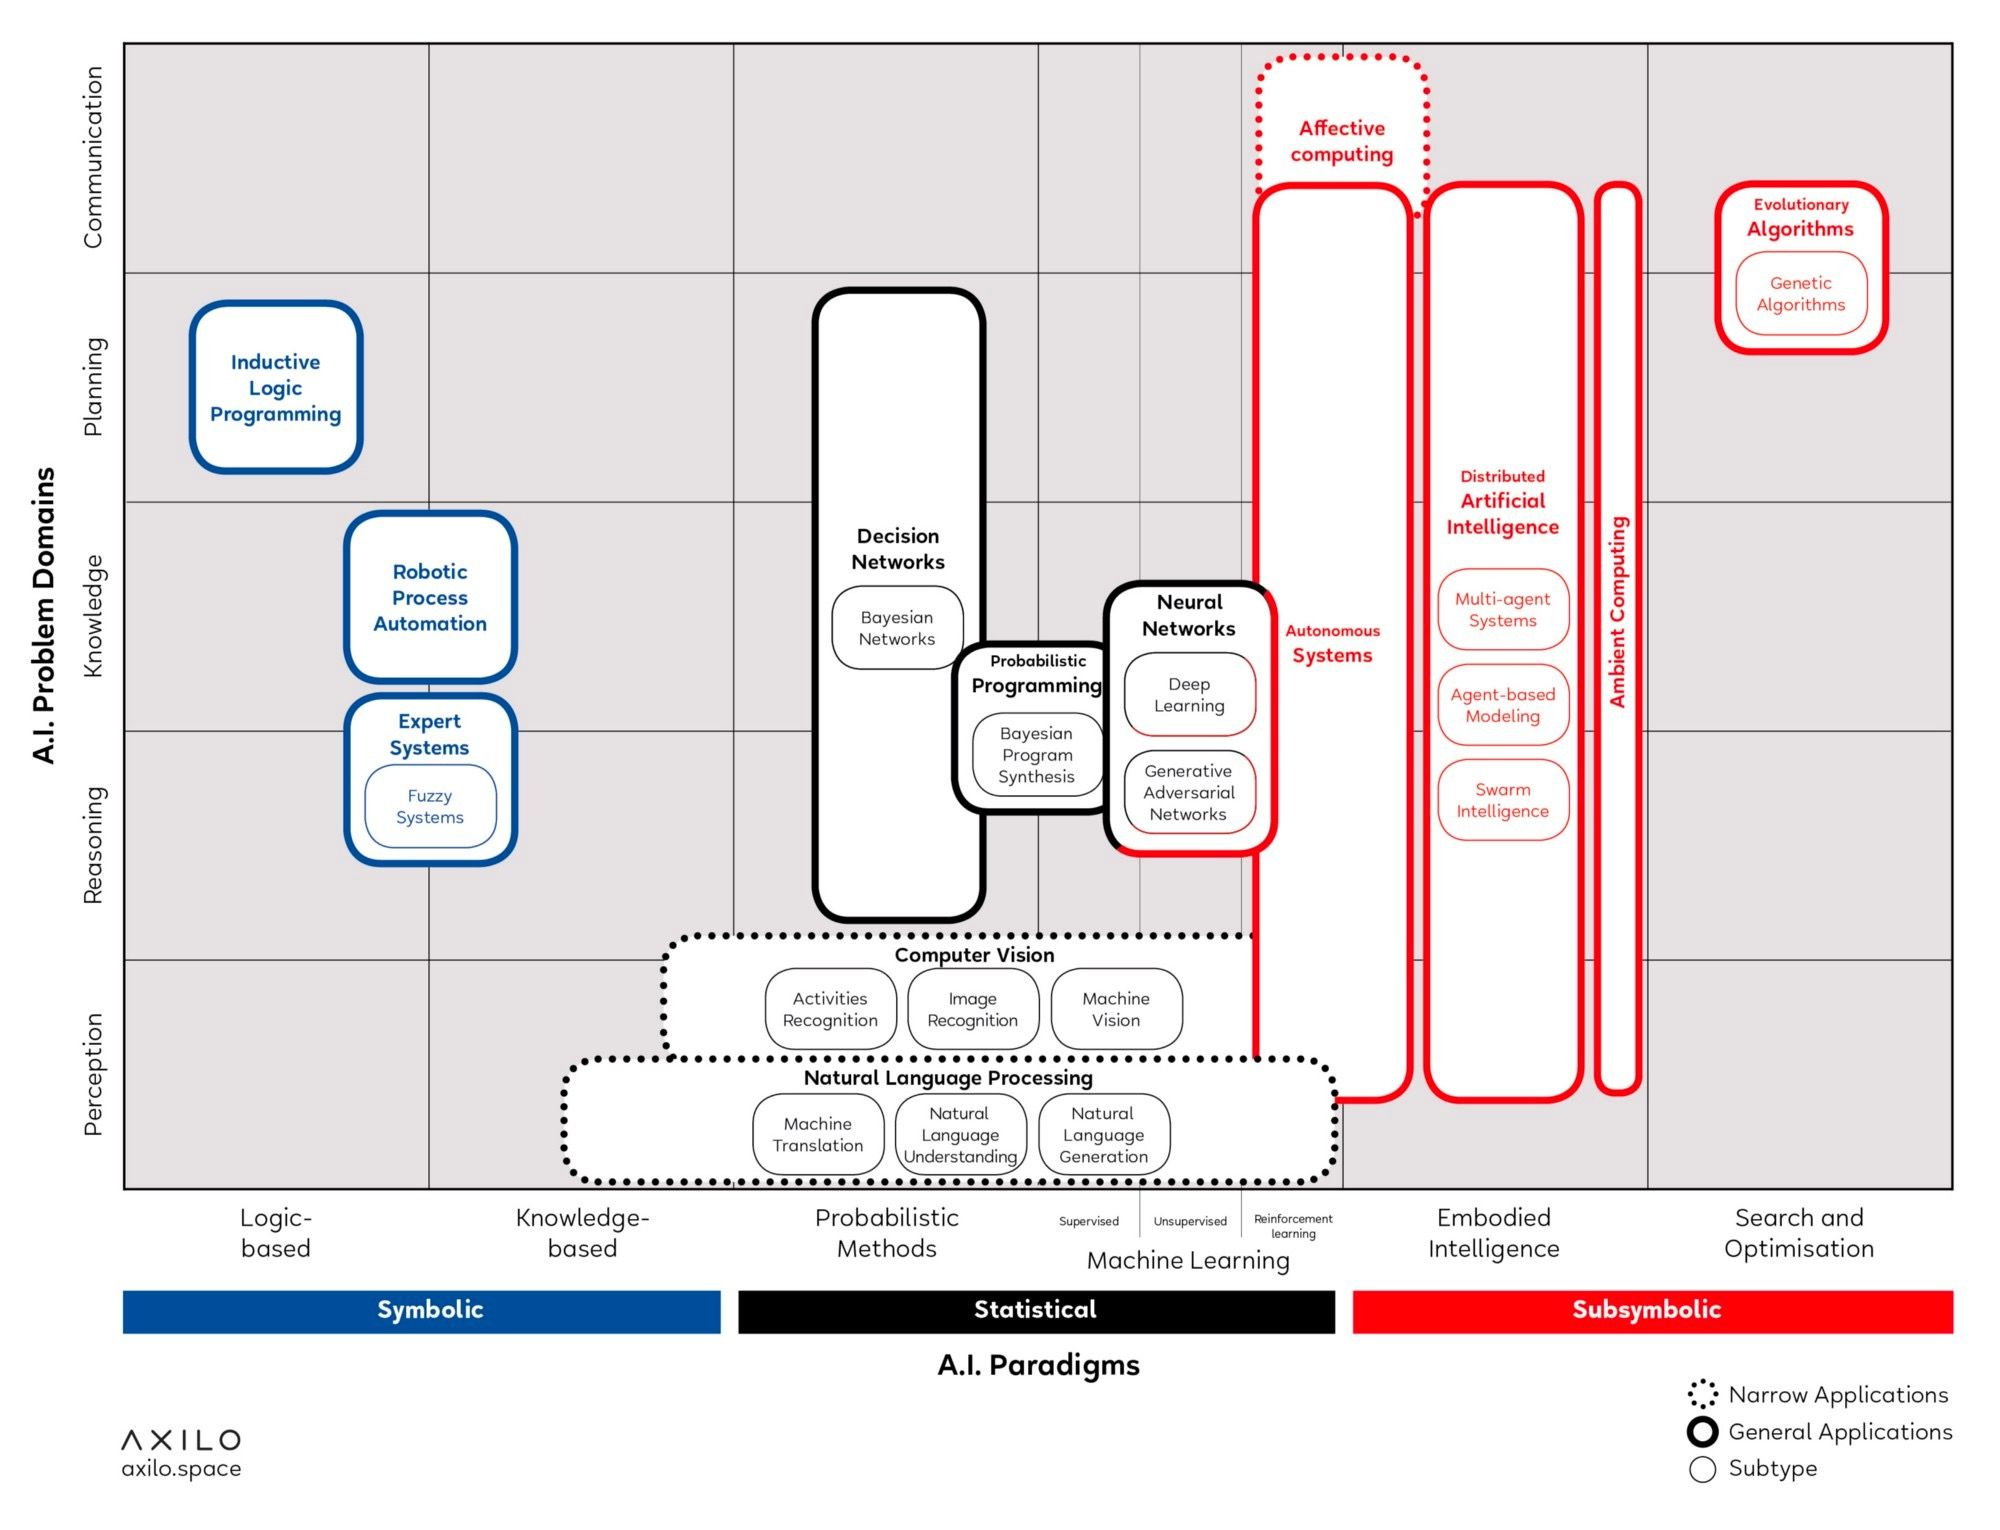
\includegraphics[scale=.23]{areas-ia.jpg}}
\end{figure}

\subsubsection{Historia}
El gran sueño del hombre ha sido siempre crear vida, por lo que hay multitud de proyectos para recrearla en forma de robots como son los geminoids. El problema con los robots que se parecen a los humanos no son sus formas humanoides, sino sus rasgos humanos que provocan el Valle inquietante (incomodidad a las personas).

Por otro lado no solo se trata de que tengan la forma sino también que se comporten como personas, es decir que sean capaces de resolver los problemas de manera parecida siguiendo un razonamiento, de ahí la Inteligencia Artificial.

Alan Turing en 1950 antes de que se acuñase el término de IA dijo:
\begin{displayquote}
	Propongo considerar la siguiente cuestión: ¿pueden pensar las máquinas?
\end{displayquote}

En la cultura popular, literatura y el cine, se ha tratado este tema muchas veces como en Frankenstein, Matrix o Terminator.

En la realidad no hay nada que se parezca a un cerebro humano, estamos muy lejos todavía de lograrlo, pero nos permite resolver ciertos problemas. Por ejemplo: Deep Blue de IBM, la RoboCup o Watson de IBM.

Estos últimos tiempos ha podido avanzar tan rápido gracias a la capacidad de cómputo (hardware) y la inmensa cantidad de datos que hay digitalizados y que se generan por segundo.

Se han hecho estudios de cuánto tiempo tardará la IA en ser capaz de reemplazar al ser humano en determinadas tareas, como escribir un best-seller, ser cirujano o un vendedor.

\subsection{Ejemplos de su uso}
\begin{itemize}
	\item Google Maps para estimar el tiempo de viaje.
	\item Filtros antispam buscando patrones similares a los clasificados como correo basura.
	\item Asistentes como Siri, Alexa o Cortana, vienen con un pre-aprendizaje para evitar sesgo.
	\item Antivirus busca patrones de comportamiento.
	\item Reconocimiento facial como en Facebook, Fotos iOS o Google Fotos.
	\item Drones repartidores para suplir la ‘last mile’, capaces de llevar cargas de un punto a otro y recargarse solos.
	\item Sistemas de recomendaciones según el comportamiento del usuario aprende sus gustos.
\end{itemize}

\subsection{Sectores que han adoptado IA mejor}
\begin{itemize}
	\item Alta tecnología y telecomunicaciones.
	\item Automovilística y ensamblado.
	\item Servicios financieros.
	\item Recursos y utilidades.
	\item Entretenimiento y media.
\end{itemize}

\section{Introducción}
En la actualidad se hace algo parecido al clásico ‘Artis Auriferae quam Chemiam vocant’ de la alquimia (química), que quiere decir El Arte de Hacer Oro que era la piedra filosofal de estos expertos, lo que les da poder.

Los profesionales de todas las áreas de la industria y los negocios buscan su particular piedra filosofal, en la actualidad el material valioso es el Conocimiento y el proceso es saber transformar los datos en conocimiento.

Los procesos que emplean los profesionales de negocios son Sistemas Inteligentes que buscan patrones no lineales, son de este tipo porque la mayoría de los problemas son. Otro punto que hace complicado encontrar patrones y relaciones en los datos es que los que se encuentren sean útiles.

\subsection{Usos}
\begin{itemize}
	\item Predicción del comportamiento del consumidor, saber que consumen los clientes para de esta manera poder captar su atención y ofrecerles oferta o productos determinados. Actualmente los usuarios buscan un producto más personalizado.
	\item Captura del conocimiento corporativo, recogen el conocimiento de profesionales con experiencia para desarrollar un sistema experto que sea capaces de realizar sus tareas.
	\item Agricultura de precisión, para optimizar el regadío, los fertilizantes o abonos, de esta manera maximizar la producción y agricultura sostenible. Se emplean robots como Wall-Ye que toma medidas de la tierra.
	\item Detección de fraudes, permiten detectar si el usuario se está saliendo de su patrón de comportamiento (conocido por todas sus transacciones), levantar una alerta y bloquear el pago.

	      El factor más importante para combatir el fraude es el Tiempo, por lo que las RNA son una gran herramienta, son capaces de detectar patrones mucho más rápido que una persona y tiene la capacidad de adaptarse.
\end{itemize}
\pagebreak

\section{Contexto}
Todo hoy en día deja un rastro de datos, incluso aunque nosotros no llevemos dispositivos electrónicos hay cámaras, tarjetas, entre muchos otros, que son capaces de recoger datos sobre nosotros.

Las grandes empresas (automotrices y financieras) fueron los primeros en darse cuenta de que esos datos son un gran activo que explotar. Los sistemas inteligentes que utilizan buscan relaciones y patrones en grandes cantidades de datos para extraer conocimiento.

Las técnicas más comunes son las Redes de Neuronas dado que hay muchas formas de estas, Algoritmos Genéticos y la lógica difusa. Antes se utilizaba en sistemas no principales, pero hoy en día está en el núcleo de la empresa ‘core-business’.

Muchas de estas técnicas están inspiradas en la naturaleza (bioinspiradas), las redes de neuronas en el cerebro, algoritmo evolutivos o inteligencia de enjambre. La pregunta es, si ha funcionado en la naturaleza, porque no imitarlo para resolver otros problemas.

\subsection{Donde se usa}
\begin{itemize}
	\item \textbf{Banca al por menor:} Evaluación de hipotecas y Predicción de demanda de productos.
	\item \textbf{Planificación:} Localización de minoristas y Distribución de productos.
	\item \textbf{Seguros:} Evaluación de riesgos y Cálculo de primas.
	\item \textbf{Marketing:} Perfiles de clientes y Venta cruzada.
	\item \textbf{Banca de Inversiones:} Predicción de activos y Gestión de cartera.
	\item \textbf{Vigilancia:} Detección de robos internos y Detección de fraudes con tarjetas de crédito.
\end{itemize}

\subsection{Motivación}
Las empresas buscan la reducción de costes, aumentar la calidad del servicio y mejora de las prestaciones del producto.

\subsection{Redes de Neuronas Artificiales}
Es una simplificación de cómo funciona el cerebro humano, su objetivo no es simular el cerebro.

Es un array de números (pesos), que dada una entrada procesa los datos y produce una salida.

\subsection{Algoritmos evolutivos}
Se codifica la solución de un problema y se genera una serie de soluciones que no tienen por qué ser buenas, solo soluciones. Después estas soluciones se mutan para dar lugar a nuevas soluciones que se evaluaran con una función para quedarnos con las mejores, el proceso se repite mejorando las soluciones progresivamente hasta llegar a la más cercana a la óptima (cuasi óptima).

Están muy orientadas a problemas de optimización.

\section{Características clave de la IA}
\begin{itemize}
	\item \textbf{Aprendizaje:} Es la característica más importante de los sistemas inteligentes. Las técnicas actuales difieren mucho de los primeros sistemas expertos, que tenían muy poca capacidad de aprender.
	\item \textbf{Adaptación:} Como todos los negocios y empresas cambian continuamente, los procesos se van quedando obsoletos, por lo que las técnicas tienen que ir evolucionando para seguir siendo útiles. Se podría reentrenar, no dejar de aprender o combinando dos procesos.
	\item \textbf{Flexibilidad:} Las decisiones humanas se caracterizan por una inherente flexibilidad, cada uno percibe las cosas de una manera distinta, pero todos lo hacemos dentro de un rango. Otra manera de expresarla es aun faltando un dato ser capaz de continuar y llevar a cabo el proceso. Los sistemas clásicos funcionan con lógica si/no.
	\item \textbf{Explicación:} Se debe saber cómo se llega a la conclusión del proceso, para poder entender como los realiza y esto permite la interacción del experto que sabrá si lo ha hecho bien. No te fiarías de una máquina que no sabes por qué dice que te tienes que operar.
	\item \textbf{Descubrimiento:} Capacidad de descubrir procesos o relaciones nuevas que no eran conocidas previamente.

	Los patrones descubiertos deben ser validados por un experto humano.
\end{itemize}

\section{Principales técnicas}
\begin{table}[H]
	\centering
	\caption{Comparativa técnicas IA}
	\resizebox{\textwidth}{!}{%
		\begin{tabular}{|c|c|c|c|c|c|}
			\hline
			Técnica                    & Aprendizaje & Flexibilidad & Adaptación & Explicación                & Descubrimiento \\ \hline
			\begin{tabular}[c]{@{}c@{}}Redes de\\ Neuronas\end{tabular} & ↑↑↑↑↑       & ↑↑↑↑↑        & ↑↑↑↑↑      & \begin{tabular}[c]{@{}c@{}}↑ \\ Suelen ser\\ cajas negras\end{tabular} & ↑↑             \\ \hline
			\begin{tabular}[c]{@{}c@{}}Algoritmos\\ Genéticos\end{tabular} & ↑↑↑↑↑       & ↑↑↑↑         & ↑↑↑↑       & ↑↑↑                        & ↑↑↑↑↑          \\ \hline
			\begin{tabular}[c]{@{}c@{}}Sistemas \\ Borrosos\\ Fuzzy\end{tabular} & ↑           & ↑↑↑↑↑        & ↑          & ↑↑↑                        & ↑              \\ \hline
			\begin{tabular}[c]{@{}c@{}}Sistemas\\ Expertos\end{tabular} & ↑           & ↑            & ↑          & \begin{tabular}[c]{@{}c@{}}↑↑↑↑↑\\ Al estar basado\\ en reglas\end{tabular} & ↑              \\ \hline
		\end{tabular}%
	}
\end{table}
También existen técnicas híbridas.

\section{Actualidad}
La Inteligencia Artificial no reemplaza a las técnicas tradicionales, pero si las enriquece o presenta alternativas.

Algunos sistemas inteligentes producen salidas que pueden ser entendidas por los que toman las decisiones.

La tendencia actual es incorporar los sistemas inteligentes dentro de otras aplicaciones de negocios, actualmente es muy accesible, pero se necesita personal. Utilización en pequeñas y medianas empresas.

Los sistemas híbridos es un área en expansión.

\chapter{Tema 2: Sistemas Expertos}
\section{Introducción}
Estos sistemas surgieron en los 70, pero proliferaron a lo largo de los 80. Se pueden llamar sistemas expertos o sistema basados en conocimiento.

Están dirigidos a resolver tareas en dominios definidos de manera limitada y que requieren conocimiento especializado, de expertos.

Llevan una larga trayectoria, en la que han aparecido numerosas variantes, y se han consolidado en muchos dominios.

\subsection{Dominios y áreas de aplicación}
\begin{multicols}{2}
	\textbf{Dominios}
	\begin{itemize}
		\item Contabilidad
		\item Finanzas
		\item Gerencia
		\item Comercialización
		\item Leyes
		\item Ingeniería
	\end{itemize}
	\columnbreak

	\textbf{Áreas de aplicación}
	\begin{itemize}
		\item Resolución de problemas
		\item Tareas de planificación
		\item Tareas en búsqueda
		\item Interpretación
		\item Monitorización
		\item Control
	\end{itemize}
\end{multicols}

\subsection{¿Qué son?}
Son programas de ordenador que exhiben un comportamiento característico de los expertos, personas que dominan un área/materia.

Son sistemas informáticos que utilizan conocimiento experto con el propósito de alcanzar un rendimiento similar al de un experto a la hora de resolver un problema muy bien definido.

Es importante destacar que los Sistemas expertos no sustituyen a los expertos, pero permiten que la experiencia y conocimiento de estos esté disponibles, lo que hace que los no expertos puedan trabajar mejor.

Son la tecnología de Inteligencia Artificial más aplicada hoy en día.

\subsection{¿Cuándo se utilizan?}
Existen unos requerimientos para aplicar un sistema experto, que son:
\begin{itemize}
	\item \textbf{Conocimiento especializado}, que provienen de expertos y libro/textos publicados.
	\item \textbf{Juicio}, la capacidad de tomar decisiones sensatas o llegar a conclusiones razonables, que tenga un criterio.
	\item \textbf{Experiencia}, contar con alguien que sepa resolver el problema para poder seguir adelante.
\end{itemize}

En relación con el problema hay dos características que debe poseer:
\begin{itemize}
	\item El problema debe ser \textbf{heurístico}, que no cuente con una solución algorítmica o al menos no fácil.
	\item El problema debe estar \textbf{bien definido}, tiene que estar claramente identificado.
\end{itemize}
Además, el área de experiencia debe estar muy definida y reconocida a nivel profesional.

Cuando se está desarrollando el sistema se necesita reclutar expertos que deseen cooperar en el desarrollo del sistema. El problema de reclutar al experto es que no quieran porque lo vean como una amenaza que les quite el trabajo.

También hay que tener en cuenta el tamaño y complejidad de la aplicación, deben ir acorde con la organización, de manera que sea manejable en función de los recursos de la organización y contando con el respaldo de la administración. Cuanto más grande y complejo más reglas requerirá.

\section{Conceptos}
\subsection{¿Qué es un sistema experto?}
Feigenbaum; McCorduck y Nii lo definen de la siguiente manera
\begin{quote}
	Los programas de IA que consiguen una capacidad a nivel de expertos en la resolución de problemas mediante la reproducción de un cuerpo de conocimiento se denominan sistemas basados en conocimiento o sistemas expertos.
\end{quote}

Lo que quiere decir que un sistema experto es: Un programa de ordenador que realiza una tarea con el nivel que alcanzaría un experto humano.

Los sistemas expertos intentas incorporar en un programa de ordenador el conocimiento de expertos humanos en un área bien definida.

Un punto clave en estos sistemas es que el dominio debe definirse de una manera limitada, no puede dar respuestas útiles a todas las posibles preguntas. Se limita a un área de conocimiento, como pasa con los expertos humanos.

\textbf{Experto:} Persona que ha desarrollado un alto nivel de habilidades que le permiten hacer juicios en un dominio específico.

Otro concepto que debemos considerar es la pericia, que es la sabiduría, práctica y experiencia en una ciencia o arte.

\textbf{Pericia:} Conjunto de capacidades que enfatizan el desempeño de los expertos humanos como extenso conocimiento de dominio, heurísticas que simplifican y mejoran los enfoques para la resolución de problemas, el metaconocimiento y la metacognición. Por último, comportamientos que permiten un mejor desempeño en una tarea determinada.

\subsection{Porque construir un sistema experto?}
Una de las principales razones de las organizaciones es que permite preservar la experiencia, los sistemas expertos almacenan una gran cantidad de conocimiento que pueden poner a disposición de personas con menos experiencia.

Otras razones son: Mejorar la productividad, hacer que la experiencia sea portable u obtener consejo de expertos que de otra manera no sería posible.

\subsection{¿Qué hace falta para construir un sistema experto?}
\begin{itemize}
	\item Lo primero es \textbf{adquirir el conocimiento}, llamado Obtención del conocimiento, que a menudo requiere una serie de entrevistas así como una observación minuciosa del experto mientras lleva a cabo sus tareas.
	\item Una vez hemos adquirido el conocimiento debemos \textbf{representar el conocimiento} de tal manera que pueda ser reutilizado por el ordenador. Existen distintas maneras:
	      \begin{itemize}
		      \item \textbf{Reglas de producción}, que son reglas del tipo Sí … Entonces …
		      \item \textbf{Marcos}, son estructuras de datos que representan situaciones estereotipadas en un dominio mediante el uso de un formalismo basado en conceptos. Se pueden considerar los predecesores de los objetos del paradigma de la Programación Orientada a Objetos.
		      \item \textbf{Redes semánticas}, que utilizan un formalismo basado en relaciones para representar el conocimiento del dominio.
		      \item \textbf{Ontologías}.
	      \end{itemize}
\end{itemize}
La representación más habitual del conocimiento para los sistemas expertos son las reglas de producción. Que tiene la forma de sí se cumple la premisa entonces se realiza la acción.

Los componentes principales para construirlo son:
\begin{itemize}
	\item La \textbf{base del conocimiento}, es una colección de hechos, reglas y procedimientos organizados en esquemas. Contiene toda la información y conocimiento sobre un campo de interés específico.
	\item Un \textbf{motor de inferencia}, cerebro del sistema, contiene las estrategias de inferencia y los controles usados por los expertos para manipular las bases de datos de conocimiento y dominio.

	      Este recibe la consulta mediante la interfaz de usuario y lleva a cabo el razonamiento en la base de conocimiento.
	\item La \textbf{interfaz de usuario}, es un componente orientado a facilitar la comunicación entre el sistema y el usuario.
\end{itemize}
También puede contener un subsistema de explicación, cuya función es contar el razonamiento llevado a cabo por el sistema experto y justificar las conclusiones alcanzas, y una memoria de trabajo reservada para descripción del problema actual y para registrar los resultados intermedios.

Otra posible estructura de sistema experto contiene además de los anteriores:
\begin{itemize}
	\item \textbf{Base de datos de dominio}, que contiene la información relevante sobre el dominio o área de interés.
	\item Un \textbf{sistema de gestión de base de datos}, que se encarga de controlar la entrada y gestionar tanto la base de datos de dominio como la base de datos de conocimiento.
	\item Un \textbf{componente de adquisición de conocimiento}, orientado a la extracción y formulación de conocimientos derivados de diversas fuentes, especialmente de expertos. En sistemas más avanzados es capaz de aprender nuevo conocimiento de manera autónoma. Permite la interacción entre el usuario y el sistema.
\end{itemize}

Un concepto importante para estos sistemas es la inferencia.

\textbf{Inferencia:} Es el proceso de encadenar múltiples reglas juntas basadas en los datos de los que se dispone. En un sistema experto lo lleva a cabo el motor de inferencia. Los mecanismos de inferencia más populares para los sistemas basados en reglas son:
\begin{itemize}
	\item \textbf{Encadenamiento hacia delante}, es una búsqueda orientada por los datos, si las cláusulas de la premisa coinciden con la situación actual el proceso intenta afirmar la conclusión.
	\item \textbf{Encadenamiento hacia atrás}, es una búsqueda orientada a objetivos, el proceso comienza con la cláusula de acción de una regla y trabaja hacia atrás a través de una cadena de reglas en un intento de encontrar un conjunto verificable de cláusulas de colisión.
\end{itemize}

\section{Herramientas de desarrollo}
Un proceso tipo para desarrollar un sistema experto incluye:
\begin{itemize}
	\item Adquisición de conocimiento.
	\item Representación del conocimiento.
	\item Selección de herramientas de desarrollo.
	\item Prototipado del sistema.
	\item Evaluación del sistema desarrollado.
	\item Proceso continuo de mejora y mantenimiento.
\end{itemize}
A la hora de seleccionar una herramienta para el desarrollo de sistemas expertos hay que tener en cuenta:
\begin{itemize}
	\item Relación costo/beneficio.
	\item Funcionalidad/Flexibilidad de la herramienta.
	\item Compatibilidad de la herramienta con la infraestructura de información existente, es un aspecto fundamental para facilitar la incorporación del sistema experto a los sistemas actuales de la organización.
	\item Fiabilidad y soporte de proveedor de la herramienta.
\end{itemize}
\subsection{Lenguajes IA}
Para comenzar el desarrollo de un sistema experto se puede hacer desde 0, diseñando y programando los componentes de un sistema experto utilizando el lenguaje de programación de propósito general utilizado en el desarrollo de sistemas basados en inteligencia artificial, como LISP o PROLOG.

Aunque también se puede utilizar lenguajes convencionales, como C, C++ o Java, que permiten dar una mayor flexibilidad a la hora de adaptar el sistema al problema de dominio específico.

Sin embargo, estos últimos lenguajes no proporcionan una idea de cómo debe ser representado el conocimiento, ni de que mecanismo deben ser diseñados para acceder a la base de conocimiento.

\subsection{Entornos híbridos}
Por otro lado, los entornos híbridos brindan mucha facilidad para la conducción de sistemas expertos, con estas herramientas personas con poca experiencia pueden trabajar con un sistema experto.

Suelen poseer una Shell de sistema experto que contiene todos los elementos esenciales de un sistema experto, exceptuando el conocimiento específico de dominio, también herramientas para construir interfaces de usuario y más características para facilitar la construcción del sistema experto.

Una Shell es una herramienta específica para sistemas expertos que facilita la implementación de estos sistemas. Además los sistemas expertos llevan mucho tiempo en el mercado, por lo que existen muchos ejemplos. El usuario introduce los parámetros de entrada al sistema y este le da salida para el problema, algunos ejemplos:
\begin{itemize}
	\item \textbf{1st-Class Fusion} brindaba un fácil acceso a la base de conocimiento e incorporaba el algoritmo ID3.
	\item \textbf{Financial Advisor} que analizaba las inversiones de capital activo como equipo e instalaciones. Fue desarrollado 1985.
	\item \textbf{KnowledgePro} es un lenguaje de alto nivel que combina funcionalidades de sistemas expertos e hipertexto. Permitía crear sistemas clásicos de reglas, si-entonces, y leer datos desde base de datos y hojas de cálculo.
	\item \textbf{Leonardo} utilizaba un lenguaje orientado a objetos llamado contract que permitía a los especialistas en marketing analizar su empresa y/o producto con respecto a la competencia.
	\item \textbf{Personal Consultant (PC) Easy} era utilizado para guiar vehículos en almacenes y plantas de manufactura.
\end{itemize}

Una Shell muy usada hoy en día es \textbf{Exsys} desarrollada por Corvid, es una herramienta diseñada para crear sistemas expertos en línea y pensada en usuarios no programadores.
\section{Aplicaciones}
Se aplican en una gran variedad de dominios con el propósito de dar soporte a la toma de decisiones. Se puede ver tanto en el área de los negocios para dar soporte como con usos médicos para el diagnóstico.
\pagebreak

Los primeros sistemas expertos estaban dirigidos al dominio de las ciencias como son:
\begin{itemize}
	\item \textbf{DENDRAL} fue desarrollada por Feigenbaum en 1965 con un razonamiento basado en reglas para deducir la estructura molecular probable de los componentes químicos orgánicos a partir de análisis de químicos conocidos y datos de espectrometrías de masas.
	\item \textbf{MYCIN} desarrollado por investigadores de la Universidad de Stanford está basado en reglas cuya finalidad era el diagnóstico médico de enfermedades bacterianas de la sangre.
	\item \textbf{XCON} es unos de los primeros sistemas expertos aplicados al área de los negocios, desarrollado por Digital Equipment Corporation, es un sistema basado en reglas para determinar la configuración óptima de los sistemas según las necesidades del cliente, era capaz de procesar el pedido en un minuto cuando el equipo de ventas tardaba 25-30 minutos.
\end{itemize}

\textbf{Áreas de aplicación de los SSEE}
\begin{itemize}
	\item \textbf{Finanzas}, que incluye análisis de créditos, evaluación de seguros, prevención de fraudes, evaluación de rendimiento, etc.
	\item \textbf{Procesamiento de datos}, que incluye selección de equipos, evaluación de proveedores y la administración de redes.
	\item \textbf{Marketing}, se aplican en la gestión de la relación con el cliente y para el análisis y planificación del mercado.
	\item \textbf{Recursos humanos}, se utilizan para la evaluación de rendimiento, programación de personal o en la gestión de pensiones.
	\item \textbf{Fabricación}, se utilizan para planificación de producción, la gestión de calidad o el mantenimiento y reparación de equipos.
	\item \textbf{Seguridad}, se han utilizado para la evaluación de amenazas terroristas y la detección de financiación de actividades de este tipo.
	\item \textbf{Automatización de procesos de negocio}, se utiliza en la gestión de call center.
	\item \textbf{Administración de la salud}, se han utilizado para resolver diferentes problemas y la aplicación en la bioinformática.
\end{itemize}
\pagebreak

\textbf{Ejemplos de Sistemas expertos}
\begin{itemize}
	\item \textbf{CoverStory} extrae información de marketing de una base de datos y redacta informes de manera automática.
	\item \textbf{ISIS-11} era utilizado por Westinghouse para programar órdenes de fabricación compleja.
	\item \textbf{CARGEX} es utilizado por Lufthansa para determinar la mejor ruta de envío de mercancía.
	\item \textbf{ACE} utilizado por AT\&T para analizar el mantenimiento de redes telefónicas.
	\item \textbf{AA, Authorizer’s Assistant}, es utilizado por American Express para la utilización de crédito para evitar riesgos a la hora de conceder crédito para disminuir las perdidas.
	\item \textbf{Escape} es utilizado por Ford Motor Company para la autorización y proceso de reclamaciones.
	\item \textbf{GURU} es una herramienta desarrollada por Micro Data Base System para dar soporte a la gerencia y análisis financiero utilizando hojas de cálculo.
	\item \textbf{XSEL} es una versión reescrita de XCON de la compañía Digital Equipment Corporation, su función es dar soporte al equipo de ventas en la configuración de los sistemas de los clientes, paso de 3 horas a 15 minutos.
\end{itemize}

Estos son solo algunos ejemplos, muchas empresas desarrollan sus propios sistemas expertos y no publican sus resultados porque son parte de su core-business.

\section{Beneficios y limitaciones}
\textbf{Beneficios de los Sistemas Expertos}
\begin{itemize}
	\item \textbf{Captura de conocimientos escasos}, se da en los casos en los que los expertos se jubilan o dejan el trabajo, pasando haber insuficientes expertos.
	\item \textbf{Aumento de la productividad y la calidad}, los sistemas expertos son capaces de trabajar más rápido que los humanos y brindar recomendaciones consistentes, reduciendo el orden de magnitud de los errores.
	\item \textbf{Disminución del tiempo de toma de decisiones}, las personas que toman consejo de sistemas expertos pueden tomar decisiones mucho más rápido.
	\item \textbf{Mejora en la resolución de problemas}, los sistemas expertos incorporan conocimiento de múltiples expertos en el proceso de análisis lo que posibilita esta mejora y la Integración de varias opiniones de expertos.
	\item \textbf{Puede trabajar con información incierta o incompleta} como lo haría un ser humano.
\end{itemize}
Estos son solo algunos de los beneficios de utilizar estos sistemas, pero también hay algunas limitaciones.

\textbf{Problemas y limitaciones de los Sistemas Expertos}
\begin{itemize}
	\item \textbf{Falta de disponibilidad del conocimiento}, puede darse el caso de que no se pueda acceder al conocimiento, que no haya expertos en el problema que queremos resolver.
	\item \textbf{Extracción de la experiencia}, es proceso difícil obtener el conocimiento de los humanos.
	\item \textbf{Miedo a compartir conocimiento}, lo sufren algunos expertos por miedo a perder su trabajo y ser remplazados.
	\item \textbf{Dominio estrecho y bien definido.}
	\item \textbf{Vocabulario técnico de los expertos.}
	\item \textbf{Falta de confianza de los usuarios finales en el sistema.}
	\item \textbf{Pueden generar recomendaciones incorrectas.}
\end{itemize}

Investigadores han hecho estudios sobre los factores que determinan el éxito o fracaso de un SSEE, son los siguientes:
\begin{itemize}
	\item \textbf{Contar con un buen gestor.}
	\item \textbf{Participación del usuario y un elemento de formación.}
	\item \textbf{Justificación de la importancia del problema de manera adecuada.}
	\item \textbf{Buena gestión de proyectos.}
	\item Es necesario que el nivel de conocimiento sea lo suficientemente alto.
	\item Debe haber al menos un experto cooperativo.
	\item El problema debe ser principalmente cualitativo.
	\item Debe ser suficientemente limitado el alcance.
	\item La interfaz de usuario debe ser de alta calidad, amigable y capaz de almacenar y manipular el conocimiento.
\end{itemize}

En 1995 se descubrió que solo un tercio de los sistemas expertos que se habían estudiado sobrevivía más allá de los 5 años, por lo general el sistema fallaba debido a problemas administrativos como la falta de aceptación del sistema por parte de los usuarios, la incapacidad de retener a los desarrolladores del sistema, problemas en la fase de transición del desarrollo al mantenimiento (falta de refinamiento del sistema), cambios en la prioridad de la organización.

Una \textbf{adecuada gestión, desarrollo y despliegue del sistema experto podría resolver la mayoría de estos problemas}.

Hoy en día no se ven muchas publicaciones sobre la aplicación de sistemas expertos, sin embargo como dice \textbf{Richard Barfus “Los sistemas expertos no desaparecieron, sino que fueron encubiertos”}, han evolucionado y se encuentran en sistemas híbridos junto a otros tipos de sistemas inteligentes.

\section{Casos}
\subsection{Caso 1: Cultivo de algodón en Pakistán}
Es un proyecto basado en el Internet de las cosas, IoT, que mediante dispositivos distribuidos y conectados que toman datos nos dan la información sobre los campos.

\textbf{Internet de las cosas (IoT)}: es la red de objetos físicos que contienen tecnología integrada para comunicarse y detectar o interactuar con sus estados internos o el entorno externo. Hoy en día todo está conectado como la lavadora, frigorífico, sensores en el campo, wearable, etc.

Otras tecnologías previas al IoT son:
\begin{itemize}
	\item Radio Frecuency Identification (RFID) es una tecnología que permite localizar objetos en un lugar.
	\item Wireless Sensor Network (WSN) que es una red de objetos interconectados dentro de una misma red para compartir datos.
\end{itemize}

Este proyecto se llevó a cabo en Pakistán porque es un país agrícola, depende mucho de su producción la economía, y se ha enfrentado a perdidas por las siguientes razones.
\begin{itemize}
	\item Siembra retrasada y baja.
	\item calidad de semilla.
	\item Peligros ambientales.
	\item Ataques de insectos y enfermedades.
	\item Riego no planificado y pérdidas de agua.
	\item Cosecha intempestiva.
	\item Uso indebido de fertilizantes e insecticidas.
	\item Falta de maquinaria y equipo.
	\item Mal manejo de cultivos maduros.
\end{itemize}

Por esto surge el proyecto de emplear tecnología para mejorar la producción. Los agricultores son en su mayoría son analfabetos, por lo que se recogerá el conocimiento de expertos y agricultores experimentados para ayudarles, el sistema se consultará a través de una app en distintas lenguas locales.

El sistema tiene como objetivo:
\begin{itemize}
	\item Manejo eficiente de cultivos. Control de riego.
	\item Advertencias y orientaciones medioambientales.
	\item Uso óptimo de fertilizantes, insecticidas y pesticidas.
\end{itemize}

El proceso que se seguirá será primero, Adquisición de conocimiento (desplegar los sensores, datos de plagas, insectos, enfermedades, maleza y entorno de crecimiento), desarrollar el sistema experto en este caso en CLIPS (reglas del tipo IF THEN ELSE) y por último los agricultores consultaran las recomendaciones del sistema.
\begin{itemize}
	\item Síntomas de insectos y recomendaciones de insecticidas.
	\item Síntomas de malezas y recomendación de plaguicidas.
	\item Síntomas de gusanos y recomendaciones de insecticidas.
	\item Programación de riego.
\end{itemize}

Los dispositivos empleados con pequeños y constan de: Sensor de suelo, Sensor de humedad, Sensor de temperatura y Sensores de humedad de la hoja. Todos estos dispositivos están conectados formando una red en la que se van comunicando la información y llega al sistema por el Gateway.

Sensores conectados > Sistema Experto > App móvil

Su estructura consta de Base de conocimiento, motor de inferencia (con agenda), Facilidad de explicación y la interfaz de usuario.

No toda la información viene de los sensores, alguna la da el propio usuario mediante la interfaz, en un futuro con una foto y visión artificial será capaz de reconocerlo por sí mismo.
\pagebreak

Conclusiones
\begin{itemize}
	\item Sistema evaluado entre julio y diciembre de 2015.
	\item Tasa de aceptación del 65 \%, en una encuesta a 100 individuos.
	\item Recomendaciones sobre riego, pestes, insectos y malezas.
\end{itemize}

Trabajos futuros
\begin{itemize}
	\item Despliegue de actuadores en campo, que sean capaces de en función de los parámetros realizarlo ellos mismos.
	\item Mejora de la funcionalidad del servidor.
	\item Despliegue de cámaras en el campo, de esta manera no se mete a mano la información.
\end{itemize}

\subsection{Caso 2: Predicción de inundaciones}
Las catástrofes meteorológicas generan inundaciones, lo que trata este proyecto es de estar prevenidos de estos mediante alertas, ya que son los que generan mayores desastres.

\textbf{Inundación:} es una condición general y temporal de anegación parcial o completa de áreas de tierra normalmente seca por el desbordamiento de aguas continentales o de marea debido a la acumulación o escorrentía inusual y rápida de las aguas superficiales de cualquier fuente.

Datos con los que cuenta
\begin{itemize}
	\item Cantidad de lluvia
	\item Duración de la lluvia
	\item Tasa de cambio en el flujo del río
	\item Nivel del agua del río
	\item Características de la cuenca de drenaje de un río (si el río es capaz de absorber el agua)
	\item Actividades humanas que se desarrolla en el área.
\end{itemize}

Se desarrolló un \textbf{sistema experto basado en reglas de creencias}, cuya estructura es:
\begin{itemize}
	\item Base de conocimiento, cuyo núcleo es la base de reglas de creencia.
	\item Motor de inferencia, realiza el razonamiento probatorio, en vez de encadenamiento hacia delante o atrás.
\end{itemize}

Se utiliza estas reglas para procesar \textbf{varios tipos de incertidumbre} en datos de sensores.
\begin{itemize}
	\item Ignorancia
	\item Incompletitud
	\item Aleatoriedad
	\item Vaguedad
	\item Imprecisión
\end{itemize}

\textbf{Las reglas tiene la forma:} Si lluviaCaida es Media Y DuraciónLluviaCaida es Alta ENTONCES CondiciónMeteorologica es {(Severa, 0), (Moderada, 0.4), (Baja, 0.6)}. Funcionan algo parecido a las reglas difusas.

Estas reglas emplean términos como Alto, Medio o Bajo, además la salida viene dada como la probabilidad de cada uno de los posibles valores de salida.

\textbf{Proceso de inferencia:} Razonamiento Probatorio
\begin{enumerate}
	\item Transformación de entrada
	\item Activación de reglas, se hace match de las reglas para ver cuál es la necesaria.
	\item Actualización de creencias
	\item Agregación de reglas
\end{enumerate}
La inferencia la hacemos de esta manera para tener en cuenta la incertidumbre.

Se van agrupando los factores de entrada generando otros factores que se van relacionando, generando una jerarquía tal que en la parte superior está la salida. La agregación de todas las reglas nos permite saber el nivel de inundación. Por ejemplo el X7 es la salida, pero depende de X8, X9, X10, X11 y X12, que son agrupaciones de entradas.

Mediante la interfaz de entrada, para cada antecedente de las reglas (no son solo las entradas, sino también las agrupaciones intermedias) se definen los intervalos de los términos difusos; alto, medio y bajo, así como el valor por defecto. Lo mismo se realiza para el consecuente.

Este sistema permite actualizar las reglas, de manera que ajusta unos pesos a cada variable de la regla para dar la salida. Se representa el conocimiento de tal manera que tenga la incertidumbre del problema, y con la llegada de las entradas voy actualizando los pesos. Se van agregando las reglas de manera que cuando todas se han lanzado se ha escalado el árbol y se conoce la predicción.

\chapter{Tema 3: Redes de Neuronas}
\section{Introducción}
Las Redes de Neuronas surgen en los años 40 con el objetivo de crear sistemas artificiales que modelen el funcionamiento del cerebro.

A continuación se presentan algunos de los nombres más importantes en la historia de las Redes de Neuronas:
\begin{itemize}
	\item \textbf{McCulloch y Pitts, 1943:} Plantearon el primer modelo matemático de red de neuronas artificiales, se basaron en que las neuronas operan mediante pulsos binarios.

	      Introdujeron el concepto de función de paso por umbral. Permitía simular comportamientos complejos a partir de cálculos muy sencillos, pero carecía de capacidad de aprendizaje.
	\item \textbf{Donald Hebb, 1949:} Se basó en dos conceptos muy importantes y fundamentales que han pasado en el campo de las redes de neuronas y que fueron obtenidos a partir de investigación psicofisiológica.

	      Primera que el aprendizaje se localiza en la sinapsis (conexiones entre neuronas) y segundo la información se representa en el cerebro mediante un conjunto de neuronas que pueden estar activas o inactivas.

	      Su aportación más importante fue el desarrollo de un procedimiento matemático de aprendizaje que se denomina Aprendizaje en Hebbiano.
	\item \textbf{Frank Rosenblatt, 1957:} Generalizado el modelo de neuronas presentado en el 43 añadiendo aprendizaje y lo llamo Perceptrón. Es la red verdadera red de neuronas más antigua.

	      Intento generalizar el aprendizaje en un modelo en tres niveles y para ello introdujo una capa oculta de neuronas, pero no logro un método matemático para entrenarla. Su perceptrón era capaz de generalizar una vez aprendidos una serie de patrones, pero no era capaz de resolver el problema XOR o problemas de clasificación no separables linealmente.
	\item \textbf{Minsky y Papert, 1969:} Publicaron una crítica muy seria al perceptrón por su naturaleza lineal que lo hacía muy limitado, que produjo una parada muy importante en la investigación denominada Época oscura.
	\item \textbf{Rumelhart, Hinton y McClelland, 1980:} Se creó el grupo de Procesamiento Paralelo Distribuido, dieron lugar a manuales muy influyentes y resurgieron el interés por las redes de neuronas artificiales.
	\item \textbf{John Hopfield, 1982:} Demostró que se puede construir una función de energía para describir la actividad de una red de neuronas monocapa en tiempo discreto. El entrenamiento de una Red de Hopfield consiste en reducir la energía de los estados que la red tiene que aprender.
	\item \textbf{Teuvo Kohonen, 1984:} Comenzó a trabajar en memorias asociativas y matrices de correlación, pero su aportación más importante son los mapas autoorganizativos, un tipo de redes de neuronas no supervisadas que usan una función de vecindad para preservar las propiedades topológicas del espacio de entrada.

	      Está formado por nodo/neuronas, para cada neurona hay un vector de pesos del tamaño de la entrada y su posición en el mapa. La distribución usual es en un espacio de dos dimensiones en forma de rejilla rectangular o hexagonal.

	      También aporto el LVQ un sistema de aprendizaje de carácter competitivo.
	\item \textbf{Stephen Grossberg, 1989:} Propuso junto a Gail Carpenter las ART (Teoría de la Resonancia Adaptativa), se trata de un tipo de redes de neuronas que son capaces de seguir aprendiendo cuando están en uso y son un modelo no supervisado.
\end{itemize}

Se usan de forma extensiva en diferentes problemas reales de muy distintas índoles.

Además, existen investigaciones recientes que han dado lugar a un nuevo paradigma, las redes de neuronas convolucionales o Deep Learning. Modelo propuesto por Yann LeCun en 1982, pero refinado en 2012 por un equipo liderado por Dan Ciresan.

\section{Definición y tipos}
Una \textbf{Red de Neuronas Artificiales} es un modelo (matemático) muy simple del conjunto de neuronas del cerebro. Se trata de conseguir el paso del circuito natural del cerebro al correspondiente circuito artificial o red de neuronas.

Las neuronas del cerebro son lentas en comparación con los circuitos eléctricos ($10^{-3}$ s y $10^{-9}$), pero las naturales realizan computo masivamente paralelo lo que reduce la apariencia de esta lentitud.

Una \textbf{neurona} es una unidad de proceso de 1 o varias entradas y con 1 o varias salidas. En la que se lleva a cabo la suma ponderada de las entradas ($a=x_1*w_1*x_2*w_2$), aplicando un peso a cada una, y se procesa mediante una función de activación ($y=F(a)$) que es la que produce la salida.

Las señales que llegan a la sinapsis son las entradas y estas señales pueden excitar a la neurona (si es positivo) o inhibirla (si es negativo). Si la suma ponderada supera un umbral se activará, si no permanecerá inactiva.

Las neuronas se encuentran distribuidas en capas, formadas por al menos 1 neurona, y estas capas están interconectadas, esto da lugar a la Red de Neuronas. La estructura de interconexión recibe el nombre de Arquitectura de la Red o Patrón de interconectividad. Las capas pueden ser: Capa de entrada, Capa oculta o Capa de salida.

Las conexiones del perceptrón están siempre orientadas hacia delante, de esta manera las neuronas de una capa se conectan con todas o algunas de las neuronas de la siguiente capa, el llamado Feedforward.

Para desarrollar una arquitectura de red se debe tener en cuenta el número de capas ocultas y su número de neuronas, que operaciones se pueden hacer en paralelo por las conexiones con la siguiente capa. Este proceso se realiza de manera manual y dependerá del problema a resolver, se está trabajando el diseño automático.

El conocimiento en las RNA se ve representado en el peso de las conexiones entre neuronas, por lo que se aprende modificando estos pesos. Cada modelo dispone de su propia técnica de aprendizaje.

\textbf{Función de activación} es una de las partes más importante de la red, esta nos permite independientemente de la arquitectura aprender relaciones no lineales de los datos. Transforma la correspondencia lineal en no lineal, las funciones más utilizadas son del tipo sigmoide, aunque se puede usar la función escalón.

\textbf{Tipos de aprendizajes}
\begin{itemize}
	\item \textbf{Aprendizaje supervisado:} Un ejemplo es el perceptrón multicapa que es capaz de aprender a partir de un conjunto de ejemplos, pudiendo aproximar funciones no lineales, filtrar ruido en los datos, etc. Este aprendizaje se ha conseguido introduciendo la capa oculta y aplicando los algoritmos de aprendizaje de descenso del error, como backpropagation.

	      Cybenko en 1989 demostró que se puede separar cualquier conjunto de datos aunque tengan relaciones no lineales siempre que se introduzca en el perceptrón una capa oculta sea del tamaño que sea.

	      Las neuronas aparecen en una red agrupadas en las tres capas mencionadas antes:
	      \begin{itemize}
		      \item Capa de entrada, las neuronas reciben información del exterior. No actúan como verdaderas neuronas, solo reciben las entradas/patrones del exterior y las propagan a la capa siguiente.
		      \item Capas ocultas, son las que realmente realizan el procesamiento de la información, comunican con la entrada y la salida. Realizan el procesamiento no lineal de los patrones recibidos.
		      \item Capa de salida, recibe información de la capa anterior y la envían hacia el exterior proporcionando la respuesta para cada uno de los patrones de entrada.
	      \end{itemize}

	      Para el aprendizaje se proporcionan a la red los datos de entrenamiento, que consisten en patrones de entrenamiento de entrada y salida, en función de la diferencia entre la salida y la salida esperada se van actualizando los pesos ($w_{i+1}=w_i+\Delta w_i$).
	\item \textbf{Aprendizaje no supervisado:} Son capaces de modificar sus parámetros internamente para adaptarse al entorno, descubriendo por si solas características, regularidades o categorías entre los datos de entrada. Proporciona de manera codificada la salida. Las neuronas y sus conexiones muestran cierta capacidad de autoorganización.
\end{itemize}

\section{Aplicaciones}
Las RNA se usan cada vez más en problemas de clasificación, predicción y clustering en ámbitos muy diversos, nosotros en la asignatura trataremos el financiero y empresarial. Algunos ejemplos son:
\begin{itemize}
	\item \textbf{Banco Mello:} Invirtió en un costoso sistema de detección de fraudes y en 6 meses habían costeado el coste del software con el ahorro en esos fraudes detectados.
	\item \textbf{Visa y Mastercard:} Monitorizan diariamente más de 1,2 millones de cuentas gracias a las RNA.
	\item \textbf{Auditorías Internas:} Se utilizan para predicción de ganancias, buscar el momento más adecuado para llevar a cabo una auditoria o gestionar estrategias en determinadas operaciones.
	\item \textbf{Ernst \& Young:} En consultoras de alto nivel, conseguir que gestores financieros mejoren la gestión del capital financiero.
\end{itemize}

En el ámbito empresarial y financiero la ventaja es que se cuenta con muchos datos pertenecientes a la empresa a lo largo del tiempo, con lo que se pueden entrenar y obtener buenos resultados.

Se siguen realizando investigaciones y por lo tanto se producen avances en su propia teoría, aunque tenga un origen antiguo (años 40) hay muchos ámbitos abiertos que estudiar. Algunos de estos ámbitos son:
\begin{itemize}
	\item Los expertos o especialistas que tratan de combinar diferentes redes de neuronas para dar lugar a los llamados \textbf{Ensembles o Conjuntos de Clasificadores}.
	\item El trabajo en \textbf{nuevos algoritmos de aprendizaje} para superar al de retropropagación, incluso en sus versiones más rápidas.
	\item \textbf{Diseño automático de arquitectura}, dado que para utilizar las RNA hay que tener un conocimiento experto, este campo está en constante estudio se trata de poder saltarnos ese conocimiento experto y que un sistema de diseño automático no indique cuál es la red de neurona más adecuada para resolver ese problema.
	\item \textbf{Nuevos modelos de RNA} como son las actuales Redes de Neuronas Convolucionales.
\end{itemize}

\textbf{Ventajas de trabajar con RNA}
\begin{itemize}
	\item Permite alcanzar unos resultados excelentes tanto en clasificación, representación o predicción, con unas tasas de acierto por encima del 98 y 99 \%.
	\item Permiten modelar y predecir comportamientos no lineales a diferencia de los métodos clásicos.
	\item Robustos pueden manejar datos incompletos, con ruido y que contienen incluso ejemplos contradictorios.
	\item Adecuadas en el procesamiento de información en finanzas y negocios.
\end{itemize}

\textbf{Desventajas de las RNA}
\begin{itemize}
	\item Son cajas negras, no son capaces de explicar cuál es la información que les ha conducido a tomar la decisión que proporciona la salida.
\end{itemize}


\section{Casos}
\subsection{Caso 1: Predicción de bancarrotas}
Un problema muy importante para las empresas y entidades financieras. Se emplean redes de neuronas en combinación con otros modelos clásicos para mejorar la predicción, como puede ser el modelo de Altman de predicción de insolvencias.

Mejoran la predicción.

Los modelos existentes son muy complejos, pero aun así incrementó su difusión y su uso según se fueron desarrollando las computadoras y hojas de cálculo.

Tradicionalmente:
\begin{itemize}
	\item \textbf{1966 Beaver:} El primero con el uso de técnicas estadísticas de univarianza. Relaciones financieras para predecir bancarrotas muchos años antes de que estas se produjeran.
	\item \textbf{1969 Altman:} Es el trabajo de referencia. Utilizo análisis mutivarianza.
	\item \textbf{1972 Edmister:} Análisis mutivarianza con análisis de tendencias.
	\item \textbf{1985 Fryman, Altman y Kao:} Utilizaron un algoritmo de particionamiento recursivo, sin embargo son modelos muy complejos que no pueden ser utilizados por personal no formado.
\end{itemize}

\subsubsection{Bankruptcy Prediction using ANN 1995: Dorsey, Edmister y Johnson}
Plantearon el uso de redes de neuronas para la predicción de bancarrotas utilizaron una serie de razones financieras de todas las que hay, que fueron razón de liquidez, solvencia/apalancamiento, endeudamiento y la razón de cobertura.

Estudiaron todas esas razones financieras para predecir bancarrotas del año 1994, estudiando las bancarrotas desde 1981-1991.

Tomaron de entrada 20 empresas de tamaño similar con activos de más de 20 millones, 10 ellas solventes y 10 que habían quebrado.

Como entradas para la red se calcularon 18 razones financieras y como salida detección de empresas saludables, de riesgo y que quebraran pronto. La salida siendo un valor entre 0 y 1, según un umbral (0.4) marcado indica el estado.

Era capaz de detectar un 100 \% de las que van a quebrar, pero falla prediciendo que no quebraron en un 30 \%.

\subsection{Caso 2: Aplicaciones en Banca}
En este ámbito tiene mucha importancia detectar cuando conceder un crédito o no, detectar fraudes, impagos, etc.

Los analistas de riesgos son los que toman estas decisiones, pero para acceder a los datos que da el banco de España son muy lento, por lo que la aplicación de redes para generar perfiles de solvencia es muy buena.

Las entradas son los valores sobre el cliente (renta, hipoteca, historial de compra, profesión, edad, etc.) y la salida si es solvente o insolvente. Esto se puede generar mediante una red de neuronas, como un perceptrón multicapas, con una capa oculta de tamaño suficiente.

Con backpropagation podrá ir aprendiendo, como entrada de aprendizaje se utilizará un 60 \% de los datos y se validará con el otro 40 \%. Esto permite que una vez entrenada al recibir un nuevo perfil sea capaz de determinar si es solvente o no.

\subsection{Caso 3: Marketing dirigido por los datos}
Se pueden utilizar redes de neuronas no supervisadas para segmentar clientes, son capaces de encontrar patrones en los datos sin haber sido entrenados para ello de manera más eficiente que los métodos de clustering clásicos.

Lo difícil es encontrar los patrones en los clientes para este marketing.

Ese caso de estudio se trata de una sociedad inmobiliaria con 5 millones de clientes y está usando una campaña por correo para promover un nuevo producto de inversión.

Ha llevado a cabo una primera campaña por correo dirigida a 50000 clientes elegidos al azar, de los que solo ha recibido respuesta positiva de 1000 de ellos (un 2 \%). El objetivo es analizar las respuestas a esta primera campaña para encontrar una manera de enfocar la campaña de forma que las respuestas se dupliquen, pasen a ser un 4 \% y conseguir 40000 nuevos inversores.

Se utilizan como entradas los datos de clientes de la base de datos, se trata de optimizarlo por lo que se usa la antigüedad del cliente (TIMEAC, tiempo que lleva abierta la cuenta en años) y su actividad de cuenta (AVEBAL, balance promedio de cuentas de los últimos 3 meses). La salida es un valor que nos tendrá que permitir diferencias el comportamiento del cliente.

Representando estas variables con respecto a si respondieron o no al correo se puede ver que no hay una clara diferencia, ambas se distribuyen de igual manera.

La puntuación de salida será 1 si contesta y 0 en caso contrario, pero los datos se solapan.

La red utilizada puede ser un perceptrón multicapa con aprendizaje supervisado, ya que la empresa conoce a los clientes y la salida. Tendría 2 neuronas en la capa de entrada, el doble en la capa oculta 4 y la capa de salida con 1 que nos dirá si contestara 1 o no 0.

Para el entrenamiento se dispone de 2000 datos de clientes, 1000 positivos y 1000 negativos.  Cada conjunto se divide en 2 conjuntos de 500. El conjunto de entrenamiento serán un grupo de 500 de los divididos, 500 positivos y 500 negativos. El conjunto de test serán los otros 1000 restantes distribuidos equitativamente.

En el entrenamiento si la red proporciona una respuesta adecuada pasa al siguiente, si se equivoca con respecto a la esperada se ajusta la red para reducir la diferencia. Esto repetido varias veces (100-500) sobre todo el conjunto de entrenamiento provoca que se vaya reduciendo el error hasta un valor aceptable.

Se puede representar de manera tridimensional, en los dos ejes la entrada y la altura la salida de la red, de esta manera podemos distinguir los que responderán y los que no.

Cuando ya está entrenando se le pasan los datos de test y se mide el error cometido por la red. Mediante la Gráfica de ganancia (Acumulado de respuestas vs. Acumulado de NO respuestas) podemos ver por encima de la bisectriz como discrimina la red.

\chapter{Tema 4: Algoritmos Evolutivos}
\section{Introducción}
“Como de cada especie nacen muchos más individuos de los que pueden sobrevivir, y como, en consecuencia, hay una lucha por la vida, que se repite frecuentemente, se sigue que todo ser, \textbf{si varía}, por débilmente que sea, \textbf{de algún modo provechoso} para él bajo las complejas y a veces variables condiciones de la vida, tendrá \textbf{mayor probabilidad de sobrevivir y}, de ser así, \textbf{será naturalmente seleccionado}. Según el poderoso principio de la \textbf{herencia}, toda variedad seleccionada tendera a \textbf{propagar} su nueva y modificada forma” \textbf{El origen de las Especies - Charles Darwin 1859}.

Empezamos con una visión general desde el punto de la biología y a partir de esta los conceptos en los que se basa la computación evolutiva, su línea temporal, elementos y características.

\textbf{Evolución:} Serie de transformaciones continuas que va experimentando la naturaleza y los seres que la componen.

\textbf{Evolución biología:} Proceso de transformación de las especies a través de cambios producidos en sucesivas generaciones.

\subsection{Historia de la Evolución}
Hasta el \textbf{siglo XVIII} no se dudaba que la naturaleza fuese inmutable, sin embargo los hallazgos de los investigadores que dieron lugar al descubrimiento de los fósiles contradecían esa naturaleza inmutable.

En el \textbf{siglo XIX, Charles Darwin y Alfred Wallace} tras varias décadas de observación y estudios realizados en distintos lugares del planeta llegaron a una misma conclusión, las especies evolucionaron a lo largo del tiempo. Ambos presentaron conjuntamente sus conclusiones a la comunidad científica en 1858, pero \textbf{Darwin fue quien publicó en 1859 su libro “El origen de las especies”} considerado el libro más influyente en la historia de la ciencia.

Hoy en día la evolución como propiedad de los seres vivos no está puesta en duda, pero si es objeto de debate los mecanismos a través de los cuales tiene lugar dicha evolución. En el siglo XX, en los años 40 se dio forma a lo que hoy se conoce como la \textbf{Teoría de Síntesis Evolutiva Moderna que recoge por un lado la selección natural de Darwin y Wallace y por otro lado la Teoría genética de Mendel base de la herencia genética, la Mutación genética como fuente de variación y la Genética de Poblaciones}.

\subsection{Computación evolutiva}
Los algoritmos evolutivos se basan en la Teoría de Síntesis Evolutiva Moderna, aplica conceptos de esta teoría para obtener una respuesta en cierto tipo de problemas.

Incorpora tres conceptos básicos de la evolución biológica, \textbf{la Selección, la Herencia y la Variación}. Desde el punto de vista de la computación \textbf{la implementación y combinación de estos tres conceptos da lugar a un algoritmo que supone un proceso de búsqueda}, por esto se utilizan principalmente \textbf{en problemas de diseño y de optimización} cuya respuesta se puede obtener mediante un proceso de búsqueda que no es viable mediante fuerza bruta o la búsqueda heurística.

\subsubsection{Historia de la Computación Evolutiva}
Esta computación empezó en los \textbf{años 50}, durante esta década se generaron prototipos computacionales de los modelos biológicos de la evolución para su análisis y validación.

En los \textbf{años 60} es cuando se traslada a la computación los conceptos de teoría de síntesis evolutiva moderna y se idean y aplican las primeras aproximaciones de los algoritmos evolutivos, dando lugar a los algoritmos genéticos, las estrategias y la programación evolutivas.

Durante 2 décadas, \textbf{los 70 y 80} apenas hubo trabajos que supusieran un avance significativo en este campo.

En los \textbf{años 90} es cuando la comunidad científica se organiza e interactúa con mucho más énfasis, organizando las primeras ediciones de diversas conferencias que hoy en día se siguen celebrando (FOGA, CEC, GECCO, etc.). Estos primeros eventos permitieron poner en común diversas ideas y teorías en busca de un mayor soporte teórico para los distintos enfoques y múltiples aplicaciones generadas hasta el momento.

\subsubsection{Características  y Aplicaciones}
La computación evolutiva es una alternativa viable para dar respuesta a problemas de \textbf{optimización y diseño} donde la elevada complejidad computacional de otros algoritmos impide obtener dicha respuesta en el tiempo requerido, también donde no se puede aplicar una heurística para obtener la solución o solución óptima.

Aplican conceptos biológicos como \textbf{cromosoma, el sobrecruzamiento y mutación del cromosoma y la selección natural}, que permiten obtener \textbf{algoritmos flexibles, fácilmente adaptables y robustos}.

\section{Elementos y características}
Se van a presentar los distintos elementos de la computación evolutiva comparados con su equivalente biológico, a continuación la correspondencia:
\begin{itemize}
	\item \textbf{Entorno natural} - Problema a resolver.
	\item \textbf{Individuo} - Una posible respuesta o solución al problema. Los individuos pueden ser representados en el espacio de soluciones determinado por la definición del problema, cada uno representa un punto de este espacio.
	\item \textbf{Población} - Conjunto de soluciones del problema, que viene limitado por el problema que estamos tratando.
	\item \textbf{Adecuación (fitness)}, capacidad de reproducirse del individuo (transferir su material genético) - Calidad de la solución, que puede ser el porcentaje de aciertos o una función determinada. Debe diferenciar de manera clara las buenas soluciones de las malas.
	\item \textbf{Cromosoma} (codificación biológica de las características del individuo y sus procesos biológicos) - Codificación de la solución (más sencillo que en la biología), los parámetros que la definen. El diseño es específico para cada problema por lo que en cada problema se diseña desde 0. La codificación puede ser binario, base 10 o alfanumérico, cada parámetro puede ser representado por más de un valor.
	\item \textbf{Gen}, unidad de información más pequeña de un cromosoma - Parte de la codificación de la solución, puede representar un parámetro completo o parte de este, si está compuesto por varios genes. Que cantidad de información representa depende de la codificación, puede ser un bit, número o letra.
	\item \textbf{Sobrecruzamiento (recombinación) y mutación} - Son operadores de búsqueda que según el problema pueden recibir modificaciones, pero consisten en:

	      El operador de sobrecruzamiento combina el material genético de dos individuos o padres para obtener nuevos individuos o hijos.

	      El operador de mutación permite realizar pequeños cambios sobre el material genético de un individuo.
	\item \textbf{Selección natural}, la selección del más fuerte o adaptado - Reutilización de buenas soluciones, no se desechan las malas, solo que tienen más probabilidad de pasar las mejores.
\end{itemize}

Una población es un conjunto de individuos que se representan cada uno mediante un cromosoma y este está compuesto por genes.

Los operadores genéticos implementan saltos dentro del espacio de búsqueda, lo que quiere decir que nos hacen explorar nuevas soluciones en busca de las mejores.

\section{Estructura básica}
La estructura que se mostrará es la estructura básica, seguida más o menos por todos, pero dependiendo del problema puede sufrir modificaciones con el objetivo de incrementar la eficacia y la eficiencia del algoritmo, que se puede reflejar en mejores respuestas, menor número de generaciones, menor número de individuos en la población.

\textbf{Pseudocódigo de la estructura básica}
\begin{lstlisting}
inicio_AE
	poblacion <- inicializarPoblacionAleatoriamente()
	obtenerValorAdecuacionPoblacion(poblacion)
	MIENTRAS ( condicionTerminacion == false )
		seleccionarPadresParaReproduccion (poblacion)
		nuevaPoblacion <- reproducirPadres (poblacion)
			//se obtiene una nueva poblacion
		obtenerValorAdecuacionPoblacion(nuevaPoblacion)
		numGeneracion <- numGeneracion + 1
		poblacion <- nuevaPoblacion
  	FIN_MIENTRAS
fin_AE
\end{lstlisting}
\begin{enumerate}
	\item Obtener de una forma aleatoria una población inicial, un conjunto de soluciones arbitrarias.
	\item Evaluamos cada uno de esos individuos, soluciones, con la función de adecuación.
	\item Modificamos la población a lo largo de generaciones.
	      \begin{enumerate}
		      \item Seleccionamos los padres a reproducir
		      \item Se reproducen los padres y se obtiene una nueva población.
		      \item Se evalúa la nueva población.
		      \item Incrementa el número de generación, si se alcanza un determinado número de generación o bien la población (individuo o subconjunto) cumple una condición se detiene, en caso contrario volvemos al paso a).
	      \end{enumerate}
\end{enumerate}

\textbf{Generar una nueva población o actualizar la población:}
\begin{enumerate}
	\item Entre la población se eligen los progenitores o padres mediante el operador de selección.
	\item A partir de los padres y mediante dos operadores, recombinación y mutación, se obtienen los denominados descendiente o hijos.
	\item Estos hijos pueden pasar a formar parte de la población siguiente en la siguiente generación.
	\item Aplicando el operador remplazo se actualiza la población.
\end{enumerate}
Este proceso se repite hasta completar la población de la siguiente generación y una vez se actualiza, se evalúa a cada uno de esos individuos.

El proceso se corresponde con un proceso de búsqueda en el que se realizan varias búsquedas en paralelo, pues se manejan diferentes soluciones alternativas que corresponden a los individuos de la población. Se realiza mediante exploración y explotación.
\begin{itemize}
	\item \textbf{Exploración:} Se corresponde a realizar grandes saltos en parte aleatorios dentro del espacio de búsqueda.
	\item \textbf{Explotación:} Consiste en realizar saltos a partir de los puntos de los individuos que suponen mejores soluciones, mejor evaluados.
\end{itemize}

Se lleva a cabo simultáneamente una búsqueda global y una búsqueda local.
\begin{itemize}
	\item \textbf{Búsqueda global:} Al considerar diferentes soluciones, con una población que trata de cubrir todo el  espacio de búsqueda, pero también se lleva a cabo al aplicar el operador de recombinación que permite a partir de los progenitores alcanzar regiones distantes del espacio de búsqueda.
	\item \textbf{Búsqueda local:} Se implementa mediante el operador de mutación, ya que supone pequeñas modificaciones sobre cada una de las soluciones.
\end{itemize}

\section{Taxonomía}
Según los distintos enfoques en los que se basan los algoritmos evolutivos se pueden clasificar en las siguientes categorías:
\begin{itemize}
	\item \textbf{Algoritmos genéticos:} Sus principios se establecieron en 1975 por Holland, considerado el padre de la computación evolutiva. A raíz de Holland y siguiendo con la teoría evolutiva otros investigadores han desarrollado los otros dos enfoques.

	      Bajo el mismo enfoque que para los algoritmos genéticos se han desarrollado ampliaciones de este enfoque dando lugar a:
	      \begin{itemize}
		      \item \textbf{Algoritmos Genéticos basados en orden:} El valor de adecuación depende del individuo, pero también de su posición y orden dentro de la población.
		      \item \textbf{Sistemas Clasificadores:} La información codificada en el cromosoma se corresponden con sistemas de reglas. Por ejemplo ayudan a tomar una decisión o a llevar a cabo el control de un sistema.
		      \item \textbf{Programación Genética:} La información del cromosoma se corresponde con programas, algoritmos o código fuente.
	      \end{itemize}
	\item \textbf{Estrategias evolutivas:} Desarrolladas por Rechenberg y Schwefel a finales de los 60 y principios de los 70.
	\item \textbf{Programación evolutiva:} Propuesta por Fogel a principios y mediados de los 60.
\end{itemize}

Algunos autores agrupan todos estos enfoques en la disciplina de Computación Evolutiva.

Todos los enfoques están abiertos de modo que se pueden modificar ligeramente o combinar entre ellos para resolver un problema de modelado o de optimización, pudiendo crear nuestro propio algoritmo evolutivo en el momento.

\subsection{Algoritmo Genético}
Es el paradigma de algoritmo evolutivo más completo, el más ampliamente estudiado y aplicado, la estructura de un algoritmo genético clásico es la vista en la sección anterior.

Se mantiene una población que:
\begin{itemize}
	\item Representa un conjunto de posibles soluciones.
	\item Esa población es sometida a transformaciones para obtener nuevos individuos.
	\item Sobre ella se aplica a un proceso de selección favoreciendo a los mejores individuos.
\end{itemize}

Tiene un componente aleatorio en las operaciones genéticas, por lo que en la búsqueda hay aleatoriedad a donde saltar y desde donde saltar.

Es un método estocástico de búsqueda ciega de soluciones cuasióptimas, por el contrario no es inherente a los algoritmos evolutivos y genéticos  utilizar elementos aleatorios a la hora de calcular el valor de adecuación de un individuo particular.

\textbf{Propiedades}
\begin{itemize}
	\item Requieren poco conocimiento del problema inicialmente.
	\item Flexibles.
	\item Fácil incorporar conocimiento o información muy específica del problema.
	\item Fácil de implementar, puesto que es un algoritmo muy sencillo de entender y modificar.
\end{itemize}

\textbf{Fases de Desarrollo}
\begin{enumerate}
	\item \textbf{Modelar el problema}, que implica:

	      \textbf{Diseñar el cromosoma} como se va a representar una solución, como se codificará y que información incluirá. Esta fase es muy dependiente del problema a resolver.

	      \textbf{Definir una función de adecuación o fitness} de modo que permita distinguir de forma significativa si una solución es mejor que otra.
	\item \textbf{Determinar de manera completa el Algoritmo Genético} se basa en el esquema general o una pequeña modificación para las que hay abundante bibliografía.

	      Diseñar a partir del esquema general el cuerpo del bucle para cada generación, los operadores genéticos de forma completa o los valores de los parámetros que definen a estos operadores.

	      Establecer la rutina de selección.

	      Diseñar e implementar los operadores de sobrecruzamiento y mutación que serán dependientes del cromosoma diseñado.

	      Determinar valores para parámetros tales como la tasa de mutación, el tamaño de la población o establecer el criterio de terminación del algoritmo genético.
\end{enumerate}

\subsection{Estrategias Evolutivas}
Fueron ideadas en los 60 especialmente para encontrar respuestas en problemas de optimización numérica.

La información codificada en el cromosoma son valores de los parámetros que definen a un sistema. Estos valores representan y codifican como datos de tipo numérico no entero, sino tipo real o float.

Los operadores que se aplican son los de selección y mutación.

La implementación de la selección a diferencia de los algoritmos genéticos es completamente determinista, puesto que se toma para generar la siguiente generación solo los mejores de la población y se desestima el resto.

Al aplicar la mutación como un gen individual se corresponde con un único valor numérico de tipo float, el valor de la mutación vendrá dado por una distribución gaussiana o normal.

\subsection{Programación Evolutiva}
No confundir con la Programación Genética.

Resulto del intento de crear o emular inteligencia artificial, en particular la programación evolutiva se concibió inicialmente como la evolución de máquinas de estado, como los autómatas finitos a través de aplicaciones sucesivas de solo el operador de mutación.

De hecho la representación de las soluciones no tiene por qué ser mediante una cadena de tokens/elementos dentro del cromosoma, sino que la solución puede ser representada tal cual es implementada.

Por ejemplo en una RNA al aplicar mutación se haría directamente sobre la matriz de pesos de la red. La mutación también podría añadir o eliminar conexiones en la red, es decir aplicar una mutación directamente sobre el fenotipo y no el cromosoma (genotipo).

No se aplica la recombinación o sobrecruzamiento, de este modo las soluciones candidatas representan lo que en el ámbito natural se llama Especies, es decir que solo se evoluciona a lo largo del tiempo mediante mutaciones.

\section{Funciones y operadores}
\subsection{Caso de Concesión de créditos}
En economía el valor de una empresa viene determinado por el valor del conjunto de sus activos.

Para un banco un préstamo concedido es un activo puesto que le supone ingresos netos positivos, sin embargo el préstamo tiene un cierto riesgo de impago y cuanto menor sea el riesgo mejor será el activo.

Por lo tanto del total de préstamos interesa minimizar el dinero perdido en la concesión de los créditos. A la hora de conceder un crédito personal, un crédito hipotecario o una reunificación de deuda se considera una serie de atributos personales, económicos y laborales de dicha persona como por ejemplo la edad, el estado civil, el número de hijos, el tipo de entidad para la que trabaja, el salario, el conjunto de deudas que pueda tener o el tiempo que lleva trabajando en la empresa.

Los bancos aplican una serie de reglas para determinar si conceden el crédito o no.

\textbf{SCORER:} Sistema en el ámbito financiero que recibe como entrada toda la información pertinente de un cliente y se obtiene como salida un valor asociado al riesgo que supondría conceder el préstamo. En función del riesgo se determina si se concede o no el préstamo y si se concede a que interés.

El scorer se compone de un conjunto de reglas (tipo if-then), que para este ejemplo será si se concede o no el préstamo. Estas reglas se pueden expresas como tabla o matriz en la que cada fila representa una regla y cada columna una característica/atributo del cliente, siendo la última si se concede o no el préstamo. De esta manera si se cumplen las condiciones de la regla se considera la respuesta de la última columna.

El \textbf{espacio de soluciones} son todas las posibles combinaciones de valores de los atributos y salida.

El \textbf{cromosoma/individuo} en este caso es la matriz entera en la que cada una de las reglas, cada gen representa un atributo y tomara tantos bits como valores posibles tenga.

10 01 010 001 010 1 / Salario Deuda Edad Hijos T.Empresa Crédito?

La \textbf{función de fitness o adecuación} se considera como un individuo todo el conjunto de reglas que supone el scorer. Para poder obtener el valor de adecuación de una matriz de reglas es necesario un histórico de créditos concedidos en el pasado donde cada uno de sus créditos se tiene la información adicional de si hubo impago o no.

El valor de adecuación refleja la cantidad de dinero que se ha perdido concediendo ese conjunto de créditos, por lo que trataremos de minimizarlo.

\subsection{Operadores}
En cada problema se pueden implementar distintas versiones de los operadores.

\textbf{Selección:} Se aplica para elegir los cromosomas que se van a reproducir, aquellos a partir de los cuales se van a obtener nuevos cromosomas. Los cromosomas con mejor valor (mayor si maximizamos o menor si minimizamos) de adecuación tienen mayor probabilidad de ser seleccionados.

\textbf{Sobrecruzamiento:} Toma el cromosoma de dos individuos distintos y genera dos nuevos recombinando trozos o genes de los cromosomas originales manteniendo el sentido del cromosoma. Se puede establecer una probabilidad para aplicar esta operación, de esta manera si no se aplica pasan los dos padres sin modificaciones. Los trozos en los que se dividen pueden deberse a 1 punto o más de corte, que se hará en el mismo gen en ambos cromosomas.

\textbf{Mutación:} Corresponde con pequeños cambios en cromosoma, que equivale a moverse poco en el espacio de búsqueda. Nos permite prevenir la saturación de la población con cromosomas similares. Consiste en una probabilidad con la que los genes de un individuo pueden sufrir modificaciones pequeñas. Si es muy alta puede desorientar la búsqueda y si es muy pequeña estancarla.

\textbf{Remplazo:} Hay diversas estrategias:
\begin{itemize}
	\item \textbf{Generacional:} Supone remplazar toda la población.
	\item \textbf{Estado estacionario:} El remplazo es parcial y se pueden aplicas distintos criterios como son remplazar los peores en fitness, remplazar los individuos progenitores o remplazar a aquellos individuos que son más parecidos entre sí en cromosoma.
\end{itemize}

\subsection{Aplicaciones}
\begin{itemize}
	\item Establecer los parámetros para el diseño del ala de un avión o de las hélices de un aerogenerador.
	\item Generación de trayectorias para robots.
	\item Diseño de redes de neuronas artificiales, como las Deep Neural Networks.
	\item Diseño de sistema de diagnóstico de fallo.
\end{itemize}

\chapter{Tema 5: Minería de Datos}
\section{Introducción}
Hoy en día la cantidad de datos que se genera diariamente es abrumadora, ya sean datos generados en las actividades cotidianas de las organizaciones, las cosas, las personas de manera consciente o inconsciente.

Para cualquier organización es vital sacar provecho de estos datos generando conocimiento y no solo almacenándolos.

El proceso  de descubrimiento de conocimiento, también conocido como Minería de datos es un factor que juega un papel fundamental a la hora de generar nuevo conocimiento y soportar el proceso de toma de decisiones.

Las empresas se enfrentan a un problema de explosión de datos desde la aparición de internet en la década de los 90 y ha ido incrementando de manera exponencial con las redes sociales y el IoT.

Aunque se tiene muchos datos el conocimiento escasea y para abordar este problema hay dos enfoques principales (no excluyentes):
\begin{itemize}
	\item Las soluciones que brindan los \textbf{entornos de administración de datos}, como el data warehousing, en particular el procesamiento analítico en línea o en laboratorio.
	\item Los \textbf{mecanismos de extracción de conocimiento} que permiten obtener reglas, regularidades, patrones, etc. Estos mecanismos se agrupan bajo el término Knowledge Discovery in Database - Descubrimiento de Conocimiento en Bases de datos.
\end{itemize}

El volumen de datos ha aumentado tanto en los últimos 50 años que es demasiado grande para aplicar solo enfoques clásicos al analizar los datos.
\begin{itemize}
	\item La estimación de número de registros es de $10^8 - 10^{12}$ con datos con muchas dimensiones ($10^2 - 10^4$ atributos)
\end{itemize}

El tamaño del \textbf{Universo digital} (cantidad de datos digitales que se crean, replican y consumen) se duplica al menos cada dos años. Se estima que en 2025 el volumen de datos ascenderá hasta los 163 zettabytes.

Es necesario usar el Descubrimiento de Conocimiento en Bases de datos (KDD) porque el crecimiento que experimentan estas bases de datos y su tasa de crecimiento hacen que no sean viables los enfoques clásicos o tradicionales para la toma de decisiones.

Muy pocos datos de los que se generan son examinados alguna vez por un ser humano por esto es fundamental el KDD para sacar partido a estos datos.

Dado el crecimiento de la base de datos una gran cantidad de consultas importantes para la organización son difícil de expresar en un lenguaje de consulta tradicional como puede ser:
\begin{itemize}
	\item Encuentra todos los casos del fraude.
	\item Encontrar todos los individuos que probablemente necesiten ayuda financiera para los estudios.
	\item Encontrar a todos los documentos que sean similares a este problema de cliente.
\end{itemize}

\section{Conceptos}
Un Proceso de Descubrimiento de Conocimiento (KDD) según Fayyad, Piatetsky-Shaphiro y Smyth “es un proceso no trivial que identifica patrones válidos, previamente desconocidos, potencialmente útiles y fundamentalmente entendibles en los datos”. Destacaremos las siguientes palabras:
\begin{itemize}
	\item \textbf{Proceso:} Implica que la minería de datos comprende muchos pasos iterativos.
	\item \textbf{No trivial:} Involucra algún tipo de búsqueda experimental o inferencia, es decir, no es tan sencillo como un cálculo de valores establecidos.
	\item \textbf{Patrones válidos:} Los patrones que se descubran deben ser siempre ciertos en nuevos datos con algún grado de certeza.
	\item \textbf{Nuevos o previamente desconocidos:} Los patrones descubiertos deben ser novedosos para el usuario dentro del contexto del dominio o el problema que se analiza.
	\item \textbf{Potencialmente útiles:} Implica que los patrones descubiertos conllevan algún beneficio para el usuario o la tarea.
	\item \textbf{Entendibles:} Deben ser compresibles, si no de manera inmediata después de un postprocesado, es decir, que el patrón debe tener sentido.
\end{itemize}

A lo largo de la historia se han utilizado muchos nombres para referirse a lo que hoy se denomina la minería de datos.

En \textbf{1960} los estadísticos usaban los conceptos \textbf{Data Fishing y Data Dredging} para referirse a la aplicación de métodos de minería de datos que pueden conducir al descubrimiento de patrones no válidos y sin sentido.

En la \textbf{década de 1990} se popularizó el término minería de datos principalmente entre estadísticos, analistas de datos y en la comunidad de bases de datos y el área de los negocios. El concepto de \textbf{descubrimiento de conocimiento en bases de datos} fue acuñado en el \textbf{año 1989} con el propósito de enfatizar que el conocimiento es el producto final de un descubrimiento basado en datos, este concepto se popularizó en los campos de IA y AA.

Existen otros nombres para denominar el proceso de encontrar patrones útiles en los datos como \textbf{arqueología de datos o cosecha de información}. En la actualidad es \textbf{más común fuera del ámbito académico usar el concepto de minería de datos}.

La minería de datos ha evolucionado y sigue evolucionando desde las intersecciones de muchas disciplinas incluyendo estadística, IA, BBDD y AA. La \textbf{meta común es extraer conocimiento de alto nivel basándose en datos de bajo nivel a partir de grandes conjuntos.}

Los datos suelen estar escondidos en \textbf{BBDD muy grandes, un almacén de datos o Data Warehouse} permite limpiar y consolidar los datos, así el almacén puede ser utilizado como fuente de datos fiable, pero no siempre es así.

Un \textbf{entorno de minería de datos suele ser un sistema cliente-servidor o una arquitectura de sistemas de información basada en Web}. Los datos son el ingrediente más crítico de la minería de datos, estos pueden incluir datos estructurados y no estructurados.

La persona que lleva a cabo el proceso de minería de datos suele ser un \textbf{usuario final con poco o ningún conocimiento de programación} pero con datos y herramientas que permiten encontrar respuestas rápidas a preguntas ad hoc. \textbf{Maximizar el rendimiento de la minería de datos} involucra, a menudo, encontrar \textbf{resultados inesperados} y requiere un \textbf{pensamiento creativo durante todo el proceso} e incluso la interpretación de los resultados.

Las herramientas de minería de datos interactúan con BBDD y hojas de cálculo así como con distintas herramientas de desarrollo lo que facilita que los datos puedan ser analizados y los resultados implementados de forma fácil y rápida. Además otros aspectos como el \textbf{procesamiento en paralelo son esenciales} para la minería de datos.

\section{Datos}
Son parte esencial en la minería de datos.

La RAE los define como: Las consecuencias derivadas de un hecho, estos pueden ser números, palabras, imágenes, notas de voz…, los datos suelen ser considerados como el nivel más bajo de abstracción, de estos se deriva la información, y de esta el conocimiento, los datos pueden ser clasificados según distintos criterios:
\begin{itemize}
	\item Estructurados, son los empleados por los algoritmos de minería de datos.
	      \begin{itemize}
		      \item Categóricos o Discretos, representan etiquetas de varias clases para dividir una variable en grupos específicos (raza, sexo, color preferido, etc.).
		            \begin{itemize}
			            \item Nominales, para códigos simples que no representan ninguna medida (estado civil)
			            \item Ordinales, etiquetas que tienen un orden entre ellos (nivel de inglés, nivel educativo)
		            \end{itemize}
		      \item Numéricos o Continuos, representan los valores numéricos de variables específicas (salario, número de hijos, temperatura, etc.), medidas continuas en una escala determinada.
		            \begin{itemize}
			            \item Intervalo, medibles en escala de intervalo (temperatura en grados Celsius en la que la ebullición es 100 y congelación 0).
			            \item Ratio, variables de medida que se encuentran normalmente en el área de la ingeniería y las ciencias físicas (Energía, Carga eléctrica, Tiempo, Masa, etc.).
		            \end{itemize}
	      \end{itemize}
	\item No estructurados o Semiestructurados, cualquier combinación de texto, imágenes, video o contenido web. Necesitan ser procesados a datos categóricos para ser usados por los algoritmos de minería de datos.
	      \begin{itemize}
		      \item Textuales
		      \item Multimedia: Audio o Imagen/Video
		      \item HTML/XML
	      \end{itemize}
\end{itemize}

Existen otras clasificaciones como datos estáticos y dinámicos, y no todos los métodos de minería de datos se pueden usar para cualquier tipo de datos estructurados, se generarían modelos incorrectos o no generar ningún modelo.

\section{Proceso}
KDD es un proceso interactivo e iterativo que involucra la toma de decisiones por parte del usuario en los pasos que conforman el proceso. Se suele seguir un proceso general, pero hay varios procesos estandarizados para la minería de datos.

\textbf{Fayyad y varios autores en 1996} propusieron un modelo de 9 pasos:
\begin{enumerate}
	\item Entender el dominio de aplicación/conocimiento previo relevante/metas del usuario final.
	\item Creación de un conjunto de datos objetivos, centrándonos en un subconjunto o muestra de datos.
	\item Limpieza y preprocesamiento de los datos, también incluye la eliminación de ruido y el manejo de datos faltantes.
	\item Reducción y proyección de los datos, encontrar los atributos que mejor representan los datos dependiendo de la tarea.
	\item Elegir la tarea de minería de datos, si es clasificación, regresión, agrupación, etc.
	\item Seleccionar los algoritmos de minería de datos.
	\item Minería de datos, que consiste en la generación de patrones  con una representación determinada por ejemplos de reglas de clasificación, árbol de decisión o modelos de regresión.
	\item Interpretación de los patrones extraídos con la posibilidad de regresar a cualquiera de los pasos del 1 al 7.
	\item Incorporar/Consolidar el conocimiento descubierto en otro sistema y documentarlo reportando a las partes interesadas.
\end{enumerate}

\textbf{Dunham en 2004} resumió los 9 pasos en tan solo 5 comenzando en la preparación de los datos:
\begin{enumerate}
	\item Selección de Datos
	\item Preprocesado
	\item Transformación
	\item Minería de datos
	\item Interpretación/Evaluación
\end{enumerate}

La industria también propuso varios enfoques como el \textbf{CRISP-DM, CRoss Industry Standard Process for Data Mining}, que es el más usado. Consta de una secuencia de 6 pasos, en la que hay gran cantidad de vueltas atrás:
\begin{enumerate}
	\item Comprensión del negocio y las necesidades del proyecto.
	\item Comprensión de los Datos.
	\item Preparación de los Datos.
	\item Modelado.
	\item Evaluación.
	\item Despliegue.
\end{enumerate}

La siguiente metodología más usada es \textbf{SEMMA, que significa Sample, Explore, Modify, Model, Assess}.

Un aspecto muy importante es el tiempo que se dedica a cada una de las fases del proceso, por lo que es importante tener una buena planificación, y la parte más costosa es la de preparación de datos.
\section{Tareas}
La  \textbf{minería de datos} construye modelos que identifican patrones, los modelos son representaciones matemáticas que identifican los patrones entre los atributos de los objetos en un conjunto de datos dado.

Un  \textbf{patrón} es una relación matemática que puede ser numérica y/o simbólica entre los elementos de datos.

Los patrones se pueden dividir en:
\begin{itemize}
	\item \textbf{Explicativos o descriptivos:} Explican las interrelaciones y afinidades entre los atributos de los datos.
	\item \textbf{Predictivos:} Predicen el valor futuro de un atributo determinado.
\end{itemize}

Los principales tipos de patrones que busca identificar la minería de datos son:
\begin{itemize}
	\item \textbf{Asociaciones}, que representan las relaciones concurrentes más comunes en las cosas. (No supervisado: A priori, OneR, ZeroR, Eclat)
	      \begin{itemize}
		      \item Análisis de enlaces (No supervisado)
		      \item Análisis de secuencias (No supervisado)
	      \end{itemize}
	\item \textbf{Predicciones}, que indican las futuras ocurrencias en determinados eventos basándose en lo que ha sucedido en el pasado. (Supervisado: árboles de clasificación y regresión, RNA, SVM, Algoritmos genéticos)
	      \begin{itemize}
		      \item Clasificación (Supervisado)
		      \item Regresión (Supervisado)
	      \end{itemize}
	\item \textbf{Clústeres}, representan las agrupaciones naturales de las cosas en función de sus características. (No supervisado: K-medias, RNA/SOM)
	      \begin{itemize}
		      \item Outliers analysis (No supervisado)
	      \end{itemize}
	\item \textbf{Relaciones secuenciales}, representan relaciones de orden temporal entre eventos.
\end{itemize}

Las tareas de minería de datos se pueden dividir en tres grupos principales, predicción, asociación y clústering.

Por otro lado, dependiendo de cómo extraigan los patrones de los algoritmos de aprendizaje se pueden clasificar en algoritmos supervisados y no supervisados.
\begin{itemize}
	\item En el caso del aprendizaje supervisado, los datos que se utilizan para entrenar incluyen tanto las variables independientes como las dependientes (los atributos y la clase).
	\item En el caso del aprendizaje no supervisado el conjunto de entrenamiento solo incluye los atributos descriptivos.
\end{itemize}

\subsection{Clasificación}
La clasificación es la tarea de minería de datos más común.

Su objetivo es analizar los datos históricos y crear un modelo que pueda predecir la clase. Al ser un método supervisado el conjunto de entrenamiento contiene instancias pre-etiquetadas o clasificadas.

Existen muchos enfoques para llevar a cabo una tarea de clasificación como árboles de decisión, redes de neuronas o métodos estadísticos como la regresión lineal.

Un método de clasificación usado comúnmente son los árboles de decisión, la idea básica es dividir recursivamente el conjunto de entrenamiento hasta que en cada decisión todos los ejemplos o casi todos pertenecen a una misma clase. De esta manera cuando recibamos una instancia iremos recorriendo el árbol hasta llegar a una hoja que será el resultado, es como ir dividiendo  el espacio de búsqueda hasta una de esas pequeñas regiones.

\subsection{Clústering}
Consiste en encontrar el agrupamiento natural de los ejemplos no etiquetados, de esta manera crea clústeres o grupos a partir de los atributos de los datos. Cuando se reciba una instancia por proximidad a los clústeres se determina cuál pertenece.

\section{Aplicaciones}
El propósito de la minería de datos en la mayoría de los dominios es resolver un problema apremiante para la organización o explorar nuevas oportunidades de negocio.

Las áreas de aplicación de la minería de datos son múltiples y diversas. Ahora comentaremos algunos ejemplos del uso de la minería de datos.
\begin{itemize}
	\item \textbf{Gestión de la relación con el cliente:} Busca crear una relación más cercana con el cliente entendiendo sus deseos o necesidades. La minería de datos puedes ser utilizada para \textbf{maximizar el retorno de las campañas de marketing}, \textbf{mejorar la retención de los clientes}, \textbf{maximizar el valor del cliente}  así como \textbf{identificar y atender a los mejores clientes}.
	\item \textbf{Banca y otros servicios financieros:} Ayuda a automatizar el proceso de \textbf{solicitud de préstamo}, \textbf{detectar fraudes}, \textbf{maximizar el valor del cliente} a través de la venta cruzada y \textbf{optimizar las reservas de efectivo} mediante la predicción de flujos de caja.
	\item \textbf{Venta al por menor y logística:} La minería de datos se puede utilizar para \textbf{optimizar los niveles de inventario} en diferentes ubicaciones, \textbf{mejorar el diseño de la tienda} en función de las relaciones de los productos vendidos, \textbf{optimizar las promociones} de ventas, \textbf{optimizar la logística} mediante la predicción de efectos estacionales y \textbf{minimizar las pérdidas debido a la vida útil} de algunos productos.
	\item \textbf{Fabricación y mantenimiento:} Se usa para \textbf{predecir fallos en maquinaria}, \textbf{identificar anomalías en los sistemas de producción} y \textbf{descubrir nuevos patrones que permitan identificar y mejorar la calidad} del producto.
	\item \textbf{Intermediación y negociación de valores:} Se puede usar la minería de datos para \textbf{predecir como y cuando cambiaran los precios} de ciertos bonos, \textbf{pronosticar las fluctuaciones bursátiles}, \textbf{evaluar el efecto de eventos en los movimientos de mercado} e \textbf{identificar y prevenir actividad de fraude}.
	\item \textbf{Seguros:} Utiliza la minería de datos para \textbf{predecir los costos de las reclamaciones}, \textbf{optimizar tarifas} en función del cliente, \textbf{optimizar el proceso de marketing} y para \textbf{predecir reclamaciones fraudulentas}.
\end{itemize}

Las áreas de \textbf{cuidado de la salud y la medicina} son las que ganan más popularidad como área de aplicación de la minería de datos.

Una de las aplicaciones más importantes de la minería de datos es el \textbf{análisis del comportamiento de los clientes}, en este proceso se llevan a cabo tareas como \textbf{predicción de la deserción}, \textbf{marketing dirigido} para la adquisición de clientes o la venta cruzada, identificar \textbf{riesgos potenciales de impago} o \textbf{detectar posibles transacciones fraudulentas}.
\begin{itemize}
	\item Ejemplo de una compañía de telefonía móvil, en 2003 tenía una tasa de deserción del 25 \%-30 \% al año y contaba con información de sus clientes.

	      La empresa toma la decisión de predecir la posible deserción en los próximos dos meses de un cliente teniendo como referencia su información de los pasados N meses.

	      Se plantea estimar el valor del cliente y establecer cuál es la mejor oferta para ofrecerle.

	      Por esas fechas Verizon Wireless era el mayor proveedor de servicios inalámbricos en EE. UU., construyó un almacén de datos de clientes y aplicó minería de datos, lo que le permitió identificar las bajas potenciales, desarrollar múltiples modelos regionales, identificar qué clientes eran propensos a aceptar una oferta y reducir la tasa de deserción de más del 2 \% a menos del 1,5 \% al mes.
\end{itemize}

Hoy en día son numerosas las áreas de aplicaciones de la minería de datos y muchos los ejemplos cualquier organización que posee datos suficientes necesita generar nuevo conocimiento a partir de esos datos ya sea para resolver problemas o explorar nuevas oportunidades tiene en la minería de datos una valiosa herramienta.

\chapter{Tema 6: Minería de Texto}
\section{Introducción}
Actualmente hay una gran cantidad de datos guardados sin ninguna estructura (se estima en un 85 y 90 \% de los datos almacenados), además crecen de forma muy rápida. Consiste en el análisis de todos estos datos \textbf{no estructurados}. 

Es importante no confundir Text mining con la recuperación de información, la recuperación de información se centra en recuperar de forma automática documentos relevantes y el Text mining se centra en la extracción de información pero de forma general. Así de esta forma podemos considerar que la minería de texto comprende varias actividades:
\begin{itemize}
	\item \textbf{Recuperar información} de los documentos o textos adecuados.
	\item \textbf{Extracción de información} que se realiza en los textos, datos claves, relaciones entre ellos, etc. 
	\item \textbf{Data Mining y Web Mining:} Permite analizar los datos para extraer asociaciones entre dichos datos clave extraídos. 
\end{itemize} 
Text Mining es un proceso semiautomático capaz de \textbf{extraer patrones de grandes fuentes de datos no estructuradas}. El que los datos no estén estructurados es \textbf{lo que lo diferencia de la minería de datos}, los elementos de entrada del proceso son documentos creados con un editor de texto, PDF, ficheros XML, etc. 

Puede verse como un proceso cuyo primer paso es dar una determinada estructura a las fuentes de datos basadas en texto para poder posteriormente extraer información relevante y conocimiento utilizando técnicas y herramientas de minería de datos.

Las áreas de aplicación en el Text mining son aquellas en las que se generan grandes cantidades de datos de texto como:
\begin{itemize}
	\item La medicina, teniendo en cuenta informes médicos.
	\item La investigación, analizando artículos de conferencias y revistas científicas.
	\item La biología, tratando documentos sobre interacciones moleculares.
	\item El derecho, considerando el proceso de distintas resoluciones jurídicas.
	\item Las finanzas, analizando informes internos de empresas.
	\item Áreas relacionadas con el correo electrónico, pudiendo filtrar spam, priorizar correos o generar respuestas de forma automática.
\end{itemize} 
Por otra parte la extracción de patrones de fuentes de texto tiene muchas y diversas finalidades:
\begin{itemize}
	\item \textbf{Extracción de información:} identificar frases relevantes y sus relaciones en un determinado texto.
	\item \textbf{Seguimiento de un determinado tema o temática (Topic tracking):} Poder predecir documentos de interés de un usuario.
	\item \textbf{Realizar resúmenes de los documentos} que pueden ser útiles a los lectores (Summarization).
	\item \textbf{Categorización (Categorization):} Clasificar documentos en una serie de categorías predefinidas en función de los temas de los documentos.
	\item \textbf{Agrupamiento de documentos similares (Clustering)}, sin un conjunto previo de categorías.
	\item \textbf{Vincular conceptos} de diferentes documentos para poder encontrar información en diferentes ámbitos (Concept linking).
	\item \textbf{Obtener respuesta a determinadas preguntas} utilizando la búsqueda de patrones similares (Question answering).
\end{itemize}

Glosario de palabras propias del área del Text Mining:
\begin{itemize}
	\item \textbf{Corpus:} Conjunto lo más extenso y ordenado posible de datos, textos científicos, literarios, etc., que pueden servir de base a una investigación.
	\item \textbf{Término:} Palabra o conjunto de palabras extraídas directamente del corpus de un dominio determinado, por medio de métodos relacionados con el procesamiento del lenguaje natural.
	\item \textbf{Concepto:} Características o aspectos clave generados de una colección de documentos utilizando algún tipo de método, así y comparándose con término podemos decir que el término concepto es un \textbf{mayor nivel de abstracción}.
	\item \textbf{Stemming:} Derivar las palabras a su raíz.
	\item \textbf{Stop Words:} Palabras que ya están previamente filtradas tanto antes como después del proceso de datos del lenguaje natural. No hay una lista universal, pero la mayoría están relacionadas con artículos, verbos auxiliares o palabras específicas del contexto que no tienen un valor útil.
	\item \textbf{Token:} Bloque de texto categorizado en una sentencia, esta categoría está relacionada con la función que dicho token representa. La asignación de significado a estos se conoce como Tokenizing.
\end{itemize}

\section{Procesamiento del Lenguaje Natural}
Los \textbf{primeros enfoques} relacionados con la minería de texto consistían en \textbf{simplificar o reducir un documento} a una colección de palabras, lo que se conoce como \textbf{bolsa de palabras (bag of words)}, así \textbf{sin considerar la gramática o el orden en el que aparecen las palabras} se podrían \textbf{clasificar o agrupar documentos}. En determinadas tareas como la detección de spam en el correo esta técnica es muy utilizada. 

Los \textbf{humanos} utilizamos las palabras \textbf{teniendo en cuenta una estructura y un orden} por lo tanto las técnicas de Text mining deben tener esto en cuenta, lo cual está relacionado con el \textbf{procesamiento del lenguaje natural}. 

El \textbf{procesamiento del lenguaje natural (PLN)} se puede considerar como un importante componente del Text Mining y se considera un subcampo de la inteligencia artificial y la computación lingüística.

Su \textbf{finalidad es entender el lenguaje natural de forma que podamos convertir texto en representaciones más formales} que un ordenador puede manejar de forma más sencilla. El problema es, que es exactamente entender o comprender un texto, ya que el lenguaje es muy ambiguo y dependiente del contexto.

Debido a esta complejidad de esta tarea se plantean varios desafíos:
\begin{itemize}
	\item \textbf{Etiquetar partes de un discurso} para lo que hay que tener mucha información sobre el contexto en el que se enmarca dicho texto.
	\item \textbf{Segmentar texto}, lo que debe tener en cuenta por ejemplo las combinaciones de palabras.
	\item \textbf{Detectar los mejores significados de una palabra}, es decir, eliminar la ambigüedad que pueda existir en determinados conceptos.
	\item \textbf{Eliminar la ambigüedad sintáctica} ya que el mismo texto puede tener significados diversos en entornos diferentes.
	\item \textbf{Detectar y solventar entradas imperfectas} teniendo en cuenta que los humanos podemos cometer errores al hablar o escribir y que estos deben considerarse en este procesamiento de texto.
	\item \textbf{Detectar sentencias que implican acciones}, ya que algo puede requerir como respuesta una acción y no una frase.
\end{itemize}

Otra de las áreas en las que el lenguaje de procesamiento natural se está aplicando está relacionado con el \textbf{análisis de sentimiento o el también conocido como minería de opinión, opinion mining}. El análisis de sentimiento es una técnica utilizada para captar el tono emocional que expresan un conjunto de palabras y detectar así opiniones o emociones. Esta técnica es muy utilizada para detectar la opinión que tiene una persona sobre un producto a partir de un conjunto de fuentes de datos de texto.

Cabe destacar que el procesamiento de lenguaje natural está siendo utilizado en una gran variedad de aplicaciones: recuperación de información, realizar resúmenes automáticos, respuesta a preguntas, conversión de bases de datos a lenguaje natural, extracción de información automática o asistencia para lectura de un texto extranjero con pronunciación y acento correcto.

\section{Proceso de Minería de Texto}
Para que un proceso de minería de texto tenga éxito debe \textbf{seguir un proceso estandarizado} (como seria CRISP-DM en minería de datos, si se usase este habría que centrarse en el preprocesado de datos). 

Lo que tienen en común todos los procesos de minería de texto es que las \textbf{entradas} deben ser tanto no estructuradas (texto) como estructurados (bases de datos).

Considerar ciertos \textbf{controles} como las limitaciones de hardware y software, los aspectos de privacidad y las limitaciones lingüísticas. Además, los \textbf{mecanismos}, que incluyen la experiencia del dominio, técnicas y herramientas apropiadas.

La \textbf{salida} será conocimiento específico del contexto, a partir de procesamiento de los datos no estructurados.

Este proceso se puede dividir en 3 tareas consecutivas, pero que pueden requerir revisar las anteriores:
\begin{enumerate}
	\item \textbf{Establecer el corpus}
	\begin{enumerate}
		\item Obtener todos los documentos relacionados con el dominio de interés que se va a estudiar (ficheros de texto, XML, emails o páginas webs).
		\item Estandarizar los documentos, se transforman estos documentos para que todos puedan ser representados de la misma manera y poder ser procesados después por un ordenador.
	\end{enumerate}
	\item \textbf{Crear la matriz término-documento:} las filas representan los documentos considerados, las columnas los términos que aparecen en dichos documentos y la relación entre estos conceptos se marca en las casillas. Los posibles valores para los índices son:
	\begin{itemize}
		\item El número de veces que aparece un término en un documento, donde los índices deben representar valores que están normalizados. $$\textit{TF-IDF}_{t,d} = TF_{t,d}\cdot IDF_t= \textit{TF Normalizado}_{t,d} \cdot \log \left(\frac {N} {d_{ft}} \right) $$. 
		\begin{itemize}
			\item TF es frecuencia del término e IDF es frecuencia del término en el corpus.
			\item $TF_{t,d}$ el número de aparición de un término $t$ en un documento $d$ y \\ $\textit{TF Normalizado}_{t,d}$ las normalizadas.
			\item $IDF_t = \log \left(\frac N d_{ft} \right)$ siendo $N$ el número de documentos y $df_t$ el número de documentos que contiene el término $t$.
		\end{itemize}
	\end{itemize}

	Aunque puede haber términos que aun apareciendo en todos los textos (artículos, verbos, etc.) no sean relevantes, son llamados stop words. 
	
	También puede haber sinónimos, pudiéndose juntar en un solo término mediante stemming.
	
	\item \textbf{Reducir su dimensionalidad:}
	\begin{itemize}
		\item Utilizar conocimiento de expertos para eliminar los términos menos relevantes.
		\item Eliminar los términos de menor frecuencia en pocos documentos.
		\item Descomposición en valores singulares (SVD) de la matriz termino-documento, este es el más difícil.
	\end{itemize}
	
	\item \textbf{Extraer conocimiento:} para ello utilizaremos distintos métodos ya conocidos.
	\begin{itemize}
		\item Clasificación, llamado Categorización de texto.
		\item Agrupamiento de documentos similares.
		\item Asociación, relación entre términos o conceptos de términos.
		\item Análisis de tendencia nos permite identificar la evolución de conceptos clave en diversos campos.
	\end{itemize}
\end{enumerate}

\section{Aplicaciones}
Remarcar que las empresas tienen grandes cantidades de datos no estructurados de los que aplicando text mining pueden extraer conocimiento, se han empezado a dar cuenta de que es un recurso valioso.
Algunas de las muchas aplicaciones que utilizan text mining son:
\begin{itemize}
	\item Marketing
	\begin{itemize}
		\item Ofrecer productos a los clientes, analizando los datos de los call centers.
		\item Opiniones de usuarios, es importante analizar la información que se puede obtener de diferentes webs de opiniones de usuarios.
	\end{itemize}
	\item Biomedicina, dado que la literatura de este campo crece exponencialmente, está muy estandarizada y organizada. La terminología utilizada es relativamente constante, siguiendo una ontología común estandarizada. 
	
	Se realizan tareas que generan grandes cantidades de datos relacionadas con los datos y las proteínas en:
	\begin{itemize}
		\item Análisis de micro-arrays de ADN
		\item Análisis de genes
	\end{itemize}
	\item Disciplinas científicas, ya que se debe extraer gran cantidad de información de muchas bases de datos, la indexación es fundamental. Distintas instituciones académicas han lanzado iniciativas relacionadas con el text mining que ayudan a los investigadores.
	\item Aplicaciones de seguridad, se puede mencionar como ejemplo el sistema de vigilancia Echenoz, considerada la mayor campaña de espionaje de la historia para interceptar comunicaciones electrónicas. También aplicado en declaraciones de criminales para saber si ciertas o falsas.
\end{itemize}

\chapter{Tema 7: Minería Web}
\section{Introducción}
La \textbf{World Wide Web conocida como web (www), es un gigantesco repositorio de datos}, hay información sobre cualquier tema. Podría considerarse como el repositorio de datos y texto más grande del mundo y además crece muchísimo cada día. Al contenido propio de las páginas web, debemos añadir información sobre búsquedas que realizan los internautas, enlaces a los que se accede, transacciones de comercio electrónico que se realizan, etcétera. 

Por lo tanto \textbf{esta información sobre la interacción del usuario con determinadas webs} también nos puede ayudar a \textbf{entender mejor la relación entre una web y los internautas} que la visitan. Teniendo esto en cuenta, son muchos los retos que se plantean para poder extraer información de forma efectiva y eficiente de esta base de datos gigantesca que es la web.

El primero de estos retos está relacionado con la \textbf{extremadamente alta cantidad de datos} que posee la web. Esto hace que recoger datos e integrarlos sea todo un reto. 

La \textbf{complejidad} de una página web es mucho mayor que la de una página de un documento de texto tradicional, y es que \textbf{no hay una estructura unificada} de las distintas páginas web.

También es un reto, el \textbf{enorme dinamismo} que tiene la web, ya que no solo debemos considerar que esta crece de forma extremadamente rápida, sino que también debemos tener en cuenta que está siendo constantemente actualizada. 

Otro reto remarcable es la \textbf{gran diversidad de las distintas comunidades} que utilizan la web y es que los usuarios de la web tenemos distinta formación, intereses o finalidades.

Por último, debemos recordar que la web tiene absolutamente todo tipo de información, por lo que extraer aquella pequeñísima parte que interesa a cada internauta es una tarea realmente compleja.

Así, teniendo en cuenta todos estos retos o problemas que debemos afrontar, podemos considerar que los \textbf{motores de búsqueda basados en término} son actualmente una gran herramienta para poder encontrar lo que buscamos en esta gran base de datos, sin embargo, una búsqueda basada en un conjunto de términos tiene ciertas deficiencias.

La primera de ellas es que ciertos temas o materias, tienen una cantidad enorme de documentos relacionados y puede que algunos documentos tengan muy poca relevancia con dicho tema. Por otra parte hay muchos documentos muy relevantes para una determinada temática, pero podrían no contener los términos por los que se busca.

De esta forma la minería web es un enfoque más relevante que un motor de búsqueda, ya que \textbf{la minería web puede ser utilizada para mejorar el potencial de estos motores de búsqueda}.

Para ello, Web Mining puede \textbf{identificar autores de determinadas páginas web}, \textbf{clasificar documentos} y \textbf{resolver ambigüedades y ciertos matices} que no puedan realizar los motores de búsqueda basados en términos.

\textbf{Minería web:} Proceso de descubrir relaciones intrínsecas de los datos web, los cuales son expresados en forma de texto, enlaces y uso de la información.

Las 3 \textbf{áreas principales} son:
\begin{itemize}
	\item Web Mining de \textbf{contenido}
	\item Web Mining de \textbf{estructura}
	\item Web Mining de \textbf{utilización}
\end{itemize}

\section{Web mining de Contenido}
Proceso de \textbf{extracción de información útil del contenido de páginas web}, tanto texto, imágenes, vídeo, audio, listas o tablas. 

En este campo podemos encontrar técnicas de otros enfoques como son la \textbf{Recuperación de la Información} (IR) o el \textbf{Procesado de Lenguaje Natural} (NLP). Este proceso de extracción de información puede dividirse en dos partes destacadas:
\begin{enumerate}
	\item \textbf{Preparación del contenido}
	\begin{itemize}
		\item Extracción de texto a partir de HTML.
		\item Realizar “stemming”.
		\item Eliminar las palabras frecuentes, conocidas como StopWords.
		\item Calcular la frecuencia de palabras en una colección (DF).
		\item Calcular frecuencia de términos por documento (TF).
	\end{itemize}
	\item \textbf{Creación del vector} representativo en función de sus términos. 
	
	Para ello, normalmente \textbf{se utiliza una técnica de recuperación de información} muy utilizada que consiste en que cada documento sea representado por un vector de pesos asociados a dichos términos. Después, se pueden utilizar técnicas para medir cómo de relevante es un término en un documento de una colección. 
	
	Una de las \textbf{técnicas más comunes es la conocida como TF-IDF}, así un peso alto en TF-IDF se alcanza con una elevada frecuencia de un término en el documento dado y una frecuencia de ocurrencia de dicho término en la colección completa de documentos. 

	TF-IDF(t, d, D) = TF(t, d)*IDF(t, D)
	
	Además, también se asignan pesos adicionales a los términos que aparecen como palabras claves o en títulos.
\end{enumerate}

En relación con las aplicaciones relacionadas con la web de contenido, podemos considerar:
\begin{itemize}
	\item La identificación de los temas representados por los documentos en una web
	\item La categorización de documentos web
	\item Encontrar páginas web similares en distintos servidores
	\item Detectar la relevancia de contenido, lo que hace que podamos mejorar las consultas estándar como las recomendaciones.
\end{itemize}

\section{Web mining de Estructura}
Proceso de \textbf{descubrir información de la estructura de la web}. Este proceso se puede llevar a cabo tanto a \textbf{nivel de documento}, lo que se conoce como \textbf{intra-page}, como a nivel de \textbf{hiperenlaces} lo que se conoce como \textbf{inter-page}. La estructura de un grafo típico de web consiste en páginas web como nodos y los hiperenlaces como arcos que conectan dos páginas relacionadas.

La motivación de este tipo de web mining se encuentra en que los hiperenlaces son útiles no solo para navegar, sino también para apuntar a páginas con autoridad en el mismo tema que la página que contiene el enlace. Así utilizando los hiperenlaces se puede recuperar información útil de la web.

Algunos de los principales conceptos de la minería web de estructura son los siguientes:
\begin{itemize}
	\item \textbf{Un grafo web:} es un grafo directo que representa la web.
	\item \textbf{Nodo:} cada página web es un nodo en este grafo web.
	\item \textbf{Enlace:} cada hiperenlace en la web es un arco en el grafo web
	\item \textbf{Grado entrante de un nodo p:} es el número de enlaces distintos que apuntan a p
	\item \textbf{Grado saliente de un nodo p:} es el número de enlaces distintos que salen de p y señalan a otros nodos.
\end{itemize}
\pagebreak

Relaciones de hiperenlaces más comunes, destacamos:
\begin{itemize}
	\item la promoción.
	\item el refuerzo mutuo.
	\item la cotización.
	\item la opción socia.
	\item la promoción transitiva.
\end{itemize}

\textbf{PageRank} es una marca registrada y patentada por Google el 9 de enero de 1999, fue desarrollado por los fundadores de Google Larry Page y Sergey Brin en la universidad de Stanford. Este algoritmo es una familia de algoritmos utilizados para asignar de forma numérica la relevancia de los documentos o páginas web, indexados por un motor de búsqueda en función de la importancia o relevancia de una determinada página.

\section{Web mining de Utilización}
Está relacionada con aquellas técnicas que pueden \textbf{predecir el comportamiento de un usuario cuando este interactúa con la web}. Los datos que generan los internautas al visitar páginas web pueden dividirse principalmente en tres tipos:
\begin{itemize}
	\item \textbf{Datos generados de forma automática} y que son almacenados en los blogs del acceso del servidor, cookies, etc.
	\item \textbf{Perfiles de usuario}.
	\item \textbf{Metadatos} tales como atributos de la propia página y datos de utilización de esta.
\end{itemize}
El análisis de información recogida por los servidores web \textbf{puede ayudar mucho a entender mejor el comportamiento del usuario}. El análisis de este tipo de datos se denomina clickstream análisis, es decir el análisis de la secuencia de clics que realiza un determinado usuario en una web. A continuación describiremos cómo es este proceso de extracción de información utilizando web mining de utilización:
\begin{enumerate}
	\item A partir de los \textbf{logs} que produce un determinado usuario en un sitio web se realiza un preproceso de datos para poder posteriormente extraer la información relevante. Esta información obtenida no solo mejora los datos del preproceso, sino que también, podrá mejorar el propio sitio web e incrementar el valor del usuario.
	
	El preproceso de la información obtenida necesita realizar varias tareas como:
	\begin{itemize}
		\item Unir datos relacionados
		\item Realizar una limpieza de los datos de forma que podamos eliminar reintentos Separar usuarios diferentes
		\item Unir distintas sesiones
		\item Filtrar datos por tiempos
		\item Eliminar páginas irrelevantes
		\item Etcétera
	\end{itemize}
	\item \textbf{Estructurar esta información} para identificar los distintos usuarios, sus sesiones, las visitas a las páginas, etcétera.
	\item \textbf{Extracción de información} estará relacionada con la extracción de patrones de utilización, es decir, patrones sobre el comportamiento de un usuario en la web a partir de las sesiones o los ficheros log de navegación, la extracción de diferentes tipos de perfiles tanto del usuario como del sitio web o de las visitas a la web y calcular el valor del cliente en función de su comportamiento en el sitio web.
\end{enumerate}
La información extraída nos será de gran utilidad para tareas de la minería de datos de la minería web tales como:
\begin{itemize}
	\item Determinar el valor de los clientes.
	\item Designar estrategias de ventas a determinados productos.
	\item Evaluar las campañas promocionales realizadas.
	\item Predecir el comportamiento de los usuarios basándose en reglas aprendidas.
	\item Presentar información dinámica al usuario basándose en sus intereses y perfiles.
\end{itemize}

\chapter{Tema 8: Lógica difusa}
\section{El concepto de borroso}
El concepto de borroso está relacionado con el \textbf{problema de representar la incertidumbre en los sistemas de reglas}. Esta incertidumbre se genera por varias causas, se pierden datos, los datos de los que se dispone sean ambiguos o contradictorios o que la representación de esos datos sea imprecisa y por último hay que considerar que las reglas de inferencia \textbf{se basan en impresiones de expertos que no son capaces de definir con certeza} la veracidad o falsedad de tal afirmación.

Los sistemas de razonamiento \textbf{se componen de un conjunto de hechos y de inferencias}. 

Los hechos abarcan \textbf{proposiciones de dos tipos}: con un solo objeto o proposiciones que relacionan varios objetos. 

Se debe introducir en el esquema de razonamiento una manera de representar incertidumbre, probabilidad, certeza. Debemos \textbf{definir como se representa la incertidumbre, como se calcula y como se propaga por las reglas}.

Un concepto borroso representa dos ideas:
\begin{itemize}
	\item \textbf{Vaguedad de los términos}. Dificultad para realizar una precisa distinción en la definición. Por ejemplo definir el término joven sobre el dominio edad.
	\item \textbf{Ambigüedad}, definida en las relaciones que se establecen de un término a varios, es decir, cuando se debe elegir entre varias alternativas, por ejemplo en un sistema de transmisión binario donde se recibe 0 o 1, cuando se recibe 0.6 se debe decidir si es un 0 o un 1.
\end{itemize}

Este modelo está inspirado en el modo de pensar de una persona, los términos requieren una función que represente la incertidumbre y tiene que quedar abiertos. Una persona no necesita un conocimiento muy exacto para realizar inferencias, se maneja con símbolos vagos sobre la realidad.

La propuesta de \textbf{Zadeh en 1964 sobre conjuntos borrosos} establece el \textbf{marco para operar} con términos vagos. 

Tradicionalmente dado un concepto A: hombres altos y dado un concepto X: José, la afirmación X es A en el ejemplo José es alto tiene un grado de verdad 1 o 0. A través de los conjuntos borrosos el concepto A se representa mediante una función de pertenencia que se representa como $M_{AX}$ que establece el grado de como utilidad (conmutabilidad?) del predicado asociado con A y el objeto X, es decir, establece el grado de verdad de la afirmación X es A.

En \textbf{1977, Sugeno aplicó el concepto “difuso” al contexto de la ambigüedad}. Dado un objeto x del Universo X y dividido dicho universo en conjuntos no borrosos A, a cada conjunto se le asigna un valor de pertenencia del objeto x al conjunto A, $G_{xA}$, que está entre 0 y 1 y representa el grado de borrosidad de la expresión x de A.

En \textbf{1978, Zadeh relacionó los conceptos de conjunto borroso y posibilidad} a través de la distribución de posibilidad inducida por un conjunto borroso.

De forma matemática un \textbf{conjunto clásico} se define de la siguiente manera: “Sea A un conjunto no borroso definido sobre x, sea v una variable sobre x, si se dice que v toma su valor en A se dice que cualquier elemento de A puede ser posiblemente un valor de v y que cualquier elemento fuera de A no puede ser valor de v.” La frase v toma su valor en A, se puede ver la inducción de una distribución de posibilidad p sobre x, que asocia a cada elemento x la posibilidad de que x sea un valor de v.

\textbf{Conjunto clásico:} $\prod(v=x)=\pi(x)=\begin{cases} 1 \textit{ si } x \in A\\  0 \textit{ en otro caso} \end{cases}$

Si A es un \textbf{conjunto borroso}, que actúa como una restricción sobre el posible valor de v, una extensión inmediata de lo dicho anteriormente es que A induce una distribución de posibilidad igual a $\mu_A$ sobre los valores de V. Como la expresión de la distribución de posibilidad es equivalente a un conjunto borroso, se puede aplicar los conceptos de lógica borrosa sobre las distribuciones de posibilidad.
 
\textbf{Conjunto borroso:} $\prod(v=x)=\pi(x)=\mu_A(x)$

\section{Conjuntos borrosos}
Se propone un robot redondo que se mueve en un espacio con obstáculos y supongamos que tiene un sensor de distancia en la parte frontal, este sensor medirá la distancia entre la parte frontal del robot y el obstáculo. La distancia medida en metros debe ser categorizada para aplicar un conjunto de reglas que permitan al robot moverse. Para establecer la categoría normal existen dos maneras:
\begin{itemize}
	\item El conjunto normal que indica que si el robot está entre 6 y 8 metros la distancia será considerada como normal.
	\item El conjunto borroso que indica que a partir de 6 metros y a medida que la distancia aumenta \textbf{se aumenta el grado de verdad} de que la distancia sea normal. Al llegar a 7 metros se considera normal con grado 1 y sigue siendo así hasta llegar a 8 metros, momento en el que el grado de verdad \textbf{desciende linealmente hasta llegar a 0} (cuando la distancia es 9 metros).
\end{itemize}
En el ejemplo anterior se observa la definición intuitiva del conjunto borroso según una variable continua, pero para empezar es mejor hacer una definición sobre un espacio discreto.
\begin{itemize}
	\item El conjunto se define sobre un \textbf{universo del discurso U que son todos los posibles valores} que pude tomar la variable.
	\item El \textbf{conjunto borroso X se define por la función de pertenencia $\mu_x$ que toma valores entre 0 y 1}. Al ser un espacio discreto la función se representa por pares que relaciona un valor del universo del discurso con la relación de pertenencia $X=\{u, \mu_X(u)\}$. Su notación como conjunto borroso discreto se lleva a cabo utilizando el operador unión + y la barra de pertenencia /.
\end{itemize}

Un caso concreto de conjunto borroso es aquel que tiene valor en un punto, ese \textbf{punto tiene pertenencia 1 y el resto pertenencia 0}, se denomina \textbf{singleton}.

\subsection{Operadores borrosos}
\begin{itemize}
	\item \textbf{Soporte}. Todos los elementos de U con pertenencia mayor que 0.
	\item \textbf{Corte} $\alpha$. $x \in A \;\;| \;\; \mu_{xA}:(X)>\alpha$. Todos los valores que tienen un valor de pertenencia superior a alpha.
	\item \textbf{Igualdad}. $A=B$ si $\mu_a(x)$ para $x\in X$. Se dice que dos conjuntos borrosos son iguales si el valor de pertenencia es el mismo para todos los puntos del universo del discurso.
	\item \textbf{Subconjunto}. $A \subseteq B$ sii $\mu_A(x)\leq \mu_B(x)$ para algún $x\in X$. Se dice que A es subconjunto de B si y solo si todos los valores de pertenencia de A son inferiores o iguales a los de B para todos los puntos del universo del discurso.
	\item \textbf{Subconjunto propio}. $A \subseteq B$ sii $\mu_A(x)\leq \mu_B(x)$ y $\mu_A\leq \mu_B$ para algún $x\in X$. Se dice que A es subconjunto propio de B si y solo si todos los valores de pertenencia de A son inferiores o iguales a los de B para todos los puntos del universo del discurso y en algún punto el valor de pertenencia A es menor que B.
	\item \textbf{Producto cartesiano}. AB $\mu_{AB}(x)=\mu_A(x)\mu_B(x)$. Se define como el producto de las funciones de pertenencia.
	\item \textbf{Complemento A'}. El conjunto complementario A’ de uno dado A es 1 menos la función de pertenencia de A. $\mu_{A'}(x)=1-\mu_A(x)$ para $x \in X$.
	\item \textbf{Unión} $A \cup B$. La unión de dos conjuntos borrosos se define como una operación para cada valor en función de las dos funciones de pertenencias que se denomina operador disyunción $\vee$. $\mu_A(x)=\vee(\mu_A(x),\mu_B(x))$ para $x\in X$.
	\item \textbf{Intersección} $A \cap B$. La intersección de dos conjuntos borrosos se define como una operación para cada valor en función de las dos funciones de pertenencias que se denomina operador conjunción $\wedge$. $\mu_{A \cap B}(x)=\wedge(\mu_A(x),\mu_B(x))$ para $x\in X$.
\end{itemize}

\section{Lógica borrosa}
En \textbf{lógica clásica} es equivalente el grado de verdad v de una proposición Q(x), al valor que toma la función característica (función de pertenencia) de todos los elementos que verifican esa proposición $P_Q(x)$.
\begin{itemize}
	\item $v(Q(x)) = P_Q(x)$
\end{itemize}

En \textbf{lógica borrosa} el grado de verdad de una proposición es el valor de pertenencia al conjunto borroso asociado a dicha proposición. De esta manera dada una proposición B sobre el universo discurso x definida mediante el conjunto borroso B, el grado de verdad de la proposición viene dado por el valor de pertenencia al conjunto borroso B.
\begin{itemize}
	\item $v(B(x)) = \mu_B(x)$
\end{itemize}

Los grados de verdad de las operaciones borrosas se establece entre los valores de pertenencia y serán funciones matemáticas.
\begin{itemize}
	\item \textbf{Función de Negación:}
	
	Propiedades: Limite clásico, Involución y Monotonía.
	\begin{itemize}
		\item Lukasiewicz: $f \neg (a)=1-a$
		\item Sugeno: $f \neg(a)=\frac{1-a}{1-\beta a}$
		\item Yager: $f \neg(a)=(1-a^\beta)^{\frac{1}{\beta}}$
	\end{itemize}
	\item \textbf{Función de Conjunción:}
	
	Propiedades: Conmutativa, Asociativa, Elemento neutro y Monotonía.
	\begin{itemize}
		\item Mínimo: $f\wedge(a, b)=\min(a, b)$
		\item Producto: $f\wedge(a, b)=a\cdot b$
		\item Diferencia acotada: $f\wedge(a, b)=\max(0, a+b-1)$
	\end{itemize}
	\item \textbf{Función de Disyunción:}
	
	Propiedades: Conmutativa, Asociativa, Elemento neutro y Monotonía.
	\begin{itemize}
		\item Máximo: $f\vee(a, b)=\max(a, b)$
		\item Suma algebraica: $f\vee(a, b)=a+b-a\cdot b$
		\item Suma acotada: $f\vee(a, b)=\min(1, a+b)$
	\end{itemize}
\end{itemize}

Las operaciones AND y OR están conjugadas, a cada función OR le corresponde otra AND. Cuando se usa la de min se debe usar la de max, cuando se usa la de producto se debe usar suma algebraica y diferencia acotada con suma acotada.
\pagebreak

Con las de implicación pasa algo parecido, depende de cómo se definan el resto de los operadores se usarán unas u otras.
\begin{itemize}
	\item Basados en $A \rightarrow B \equiv \neg A \vee B$
	\begin{itemize}
		\item Kleene-Dienes: $\mu_{A\rightarrow B}(x, y)=\max(1-\mu_Q(x),\mu_B(y))$
		\item Lukasiewicz: $\mu_{A\rightarrow B}(x, y)=\min(1, 1-\mu_Q(x)+\mu_B(y))$
	\end{itemize}
	\item Basados en $A \rightarrow B \equiv A \wedge B$
	\begin{itemize}
		\item Mamdani: $\mu_{A\rightarrow B}(x, y)=\min(\mu_A(x),\mu_B(y))$
		\item Producto: $\mu_{A\rightarrow B}(x, y)=\mu_A(x)\cdot \mu_B(y))$
	\end{itemize}
\end{itemize}

\section{Inferencia borrosa}
En \textbf{lógica tradicional} la inferencia basada en el Modus Ponens se describe por el grado de verdad de la expresión A AND (A=>B).
\begin{itemize}
	\item Si x es A es verdad y A=>B entonces se obtiene que B es verdad. 
	\item S x es A* (algo parecido a A) es verdad el resultado es B falso.
\end{itemize}

En \textbf{lógica borrosa} se utiliza el patrón de inferencia borrosa conocido como \textbf{Regla Composicional de Inferencia de Zadeh o Modus Ponens borroso}.
\begin{itemize}
	\item Sean los conceptos A y B definidos mediante los conjuntos $\mu_A(x)$ y $\mu_B(y)$, respectivamente y la regla “SI x es A ENTONCES y es B”, si se sabe que x es A* definido como $\mu_{A*}(x)$ se puede concluir, usando MAX-MIN (OR-AND) y la implicación de Mamdani,  y haciendo el supremo de la expresión para x que $\mu_{B*}=Sup\{\min \{\mu_{A*}(x),\min \{\mu_{A}(x), \mu_{B}(x)\}\}\}$. Sale de:
	\begin{itemize}
		\item A AND (A=>B) $\min\{\mu_A(x), \mu_B(y)\}$
		\item A* AND (A=>B) $\min\{\mu_{A*}(x), \mu_B(y)\}$
	\end{itemize}
\end{itemize}

Se puede explicar esta función de forma gráfica, la función lógica implicaba definir una función f(x)=y donde el A* es el valor de entrada en el eje x y para calcular la salida se siguen tres pasos:
\begin{itemize}
	\item Se proyecta la entrada sobre la función
	\item Se calcula la intersección
	\item Se proyecta el resultado sobre el eje de salida
\end{itemize}

$$\mu_{B*}=Sup\{\min \{\mu_{A*}(x),\min \{\mu_{A}(x), \mu_{B}(x)\}\}\}=Sup\{\min \{\min \{\mu_{A*}(x), \mu_{A}(x)\},\mu_B(y)\}$$

\section{Sistema de razonamiento borroso}
Este tipo de sistemas se construyen mediante \textbf{reglas que indican la relación entre un conjunto de hechos de entrada y un conjunto de hechos de salida}. De forma más general, un sistema borroso es un sistema de reglas que relaciona un conjunto de variables de entrada con variables de salida. 

Las \textbf{variables de entrada y salida se denominan variables lingüísticas} y se definen mediante un conjunto de etiquetas. 
\begin{itemize}
	\item Una variable lingüística de entrada puede ser distancia a un obstáculo y las etiquetas pueden ser muy cerca, cerca, normal, lejos y muy lejos. 
	\item Una variable lingüística de salida puede ser velocidad y las etiquetas pueden ser muy despacio, despacio, normal, rápido y muy rápido.
\end{itemize}  

Las reglas que las relacionadas serán del estilo, SI distancia es lejos ENTONCES velocidad es alta.

Un \textbf{sistema real recibe variables con valores numéricos y da como resultado valores numéricos}, para introducir los números y proposiciones se utilizan \textbf{dos procedimientos}: 
\begin{itemize}
	\item \textbf{Fuzzyfication o Emborronado} que consiste en introducir el valor numérico y calcular el grado de pertenencia a cada etiqueta.
	\item \textbf{Defuzzification o Desembocado} que consiste en dado un conjunto de etiquetas que están activadas por diversas alturas para la misma variable, se llevan los valores de pertenencia de las etiquetas de entrada a las etiquetas de salida, mediante las reglas  se obtiene un valor numérico.
\end{itemize}

En resumen, la \textbf{realidad se mide con valores numéricos} que se \textbf{emborronan para pasarlo a los niveles lingüísticos} obteniendo el parecido \textbf{Adecuación} de cada valor con las etiquetas de la variable correspondiente, \textbf{se aplica la inferencia borrosa} y se \textbf{Agregan todos los valores} de activación de las variables de salida, mediante \textbf{desborrosificar} se obtiene nuevamente los valores numéricos.
\begin{itemize}
	\item \textbf{Fuzzificación o Grado de compatibilidad}, sobre cada etiqueta de cada variable se calcula el Grado de pertenencia o el Grado de verdad o el Grado de activación del valor medido sobre el conjunto borroso que define la etiqueta. 
	
	Si se tienen varios sensores, se calcula el grado de pertenencia para cada etiqueta (cerca, media y lejos).
	\item \textbf{Medir la adecuación de las reglas}, aplicando un operador de conjunción o disyunción, según sea la naturaleza del antecedente (and/or), sobre los hechos de la parte izquierda de la regla, de esta manera sabremos el grado de pertenencia de la regla.
	\item \textbf{Inferencia borrosa}, produce un conjunto borroso, que resulta de aplicar un operador de inferencia entre la adecuación de la regla y el conjunto borroso de la conclusión C (con función de pertenencia $\mu_C(z)$). Los operadores más típicos son el mínimo $\mu_{C}(z)=\min(a, \mu_{C}(z))$ y el producto $\mu_{C}(z)=a\cdot \mu_{C}(z)$. 
	
	Cuando se aplican varias reglas se reciben varios valores de pertenencia para la misma etiqueta, por lo que aplicamos Agregación.
	\item \textbf{Agregación}, para cada variable conclusión se agregan los resultados de todas las reglas aplicando un operador, normalmente el máximo. $$\mu_{C}(z)=\max(\mu_{C1}(z), \mu_{C2}(z), ..., \mu_{Cm}(z))$$
	
	Normalmente se combina con un operador min o prod en el paso anterior y se habla de sistemas con el Método Max-Min o Método Max-Prod.
	\item \textbf{Desfuzzificación}, es el método para transformar las etiquetas de salida de una variable en un solo valor numérico y se puede hacer mediante:
	\begin{itemize}
		\item Centro de gravedad.
		\item Centroides.
		\item Singletons.
		\item Métodos de Máxima Pertenencia: El Primero, el Último o la Media de Máxima Pertenencia (MoM).
		\item Sugeno-Tagaki: El método emplea reglas de inferencia con la siguiente estructura: IF x is A and y is B THEN z=ax+by+c donde A, B son conjuntos difusos. Se ponderan las entradas con el grado de activación.
	\end{itemize}
\end{itemize}

\chapter{Tema 9: Agentes}
\section{Introducción a los sistemas multiagentes}
El concepto de sistemas multiagentes apareció en los años 90 de la fusión de diversas disciplinas científicas como son inteligencia artificial, psicología, ingeniería de software, bases de datos, sistemas distribuidos y de la sociología.

\subsection{¿Por qué surgen?}
Se necesita construir \textbf{aplicaciones complejas} compuestas de multitud de subsistemas que interaccionan entre sí.

La división de agentes y técnicas multiagente permite la \textbf{gestión inteligente de un sistema complejo} coordinando los distintos subsistemas que lo componen e integrando objetivos particulares de cada subsistema en un objetivo común.

\subsection{¿Para qué?}
\begin{itemize}
	\item Porque algunos problemas son físicamente \textbf{distribuidos}.
	\item Cuando la complejidad de la solución requiere de \textbf{experiencia muy heterogénea}.
	\item Cuando el problema a resolver está definido sobre una \textbf{red de ordenadores}.
	\item Cuando la complejidad del problema es tal que se requiere plantear la solución de \textbf{distintos puntos de vista}.
	\item Cuando el sistema de \textbf{adaptarse} a cambios en la estructura o en el entorno.
	\item La propia \textbf{metodología} de construcción de aplicaciones está evolucionando hacia la consideración de unidades autónomas
\end{itemize}

\subsection{Características de los Sistemas Multiagentes (MAS)}
\textbf{Existe una colección de agentes} definidos a cada uno de ellos por sus propias habilidades: Adquisición de datos, Comunicación, Planificación y Actuación.

El conjunto de \textbf{todos los agentes tienen asignada una misión} que puede descomponerse en diferentes tareas independientes de forma que se puedan ejecutar en paralelo. Debe ser capaz de asignarse las tareas apropiadas a cada uno en función de la adecuación del agente a esa tarea y a la realización de la misión en común.

Cada \textbf{agente tiene un conocimiento limitado} esta limitación, puede ser tanto del conocimiento del entorno, como de la misión del grupo o de las intenciones de los demás agentes a la hora de realizar sus propias tareas.

Cada \textbf{agente tiene una mayor facilidad para hacer determinadas tareas} en función de lo que conoce la capacidad de proceso la habilidad requerida.

\subsection{Ventajas de los MAS}
\textbf{Mantener la autonomía de cada nodo de la red}, porque los nodos no dependen de la conexión con otros nodos para realizar una priorización de sus tareas cada uno de los nodos decide en función de su propio entorno las tareas más relevantes.

\textbf{Las decisiones internas se toman individualmente} con los datos internos propios del nodo, no es necesario que toda la información del sistema se encuentre en un único nodo.

\textbf{Se descarga a un hipotético sistema central de la gestión de todo el sistema}, existen agentes en los que se pueden tomar decisiones que involucran a todos los agentes. El proceso de comunicación deberá atender a estas necesidades dotando de especial importancia a algunas de las decisiones, la mayoría de las decisiones deberán ser consensuadas entre los agentes.

La \textbf{cooperación entre los distintos nodos se realiza de manera explícita}, mediante la comunicación de las necesidades de cada nodo.

La \textbf{organización entre los nodos es dinámica} lo que permite una rápida adecuación de los nodos a la situación real de todo el sistema.

La información no estará centralizada en un único punto lo que hace que el sistema sea más \textbf{robusto frente a situaciones de fallos}.

\section{¿Qué es un agente?}
Un agente es un sistema informático situado en algún entorno dentro del cual actúa de forma autónoma y flexible, para así cumplir sus objetivos.

\subsection{Propiedades básicas}
\begin{itemize}
	\item \textbf{Autonomía}: el agente es capaz de actuar por sí mismo su interacción permanente con el usuario.
	\item \textbf{Sociabilidad}: el agente es capaz de interactuar con otros agentes mediante la comunicación de información.
	\item \textbf{Reactividad}: el agente es capaz de reaccionar ante cambios imprevistos en el entorno
	\item \textbf{Iniciativa}: el agente es capaz de actuar en función de sus propios objetivos.
\end{itemize}

\subsection{Arquitectura de un agente}
Los mecanismos que permiten interconectar los componentes tanto software como hardware que hacen que un agente se comporte como tal. Se especifica cómo se descomponen los agentes en un conjunto de módulos que interactúan entre sí para lograr la funcionalidad requerida. 

Se habla de los distintos métodos de descomposición del trabajo en tareas particulares. Cómo descomponer tareas en acciones. 

Planificación y agencia estudio de mecanismos que permitan organizar la ejecución de acciones.

\subsubsection{Tipos de Arquitecturas}
\begin{itemize}
	\item \textbf{Arquitectura deliberativa}: Se caracteriza por la representación simbólica del conocimiento. Está basada en la teoría clásica de planificación, se parte de un estado inicial de partida donde existen un conjunto de planes y un estado objetivo a satisfacer. El sistema de planificación determina qué pasos se deben de llevar a cabo para conseguir sus objetivos.
	\item \textbf{Arquitectura reactiva}: Se caracteriza por no tener como elemento central de razonamiento un modelo simbólico, por lo tanto no utiliza razonamiento simbólico complejo. Manejan jerarquías de tareas que definen un comportamiento.
	\item \textbf{Arquitectura híbrida}: Se caracteriza por su estructuración por capas, generalmente en tres niveles o capas. 
	\begin{itemize}
		\item \textbf{Reactivo (bajo nivel)}: Decisiones basándose en los estímulos recibidos del entorno en tiempo real.
		\item \textbf{Conocimiento (nivel intermedio)}: Se centra en el conocimiento que se posee del medio representación simbólica.
		\item \textbf{Social (alto nivel)}: Maneja aspectos sociales del entorno incluyendo tanto información de otros agentes como deseos, intenciones, etcétera.
	\end{itemize}
\end{itemize}

\subsection{Arquitecturas de agentes}
Un agente puede verse como un sistema capaz de definirse mediante posturas intencionales donde interviene el concepto de actitud. 
\pagebreak

Las actitudes que proporcionan información (actitudes de información) están relacionadas con el conocimiento que un agente tiene sobre su entorno.
\begin{itemize}
	\item Creencias
	\item Conocimiento
\end{itemize}
Las pro-actitudes son aquellas que guían de algún modo las acciones del agente.
\begin{itemize}
	\item Deseo
	\item Intención
	\item Obligación
	\item Compromiso
	\item Elección
	\item …
\end{itemize} 

Cuál es la combinación de actitudes más adecuadas para caracterizar los agentes ha sido discutido por diferentes autores que han propuesto diferentes modelos para representar las actitudes.
\begin{itemize}
	\item Conocimiento y acción: Moore (1990)
	\item Intención: Cohen y Levesque (1990) utilizan dos actitudes básicas, creencias y objetivos
	\item Creencias, Deseos, Intenciones: Rao y Georgeff (1991)
	\item Intenciones, Creencias, Conocimiento, Saber-Como: Singh (1994)
\end{itemize}

El modelo más conocido es el Modelo BDI (Creencias, Deseos e Intenciones)

\subsection{Modelo BDI}
\textbf{Las creencias} representan el conocimiento que se tiene del entorno. Representar el estado del entorno, recordar eventos pasados, recordar el ámbito de percepción, almacenar información importante para evitar el tener que recalcularla a partir de la información previa, representar información imperfecta. 

\textbf{Los deseos} son los objetivos del agente, es el valor de una variable un registro o una expresión simbólica en alguna lógica. Representa algún estado final deseado, ya que el software convencional está orientado a la tarea en lugar de al objetivo de forma que cada tarea o su rutina se ejecuta sin ningún recuerdo de por qué ha comenzado su ejecución.

Son suficientes las creencias y los objetivos si se ha decidido llevar a cabo una acción un plan y el entorno cambia de alguna forma que se haría, continuar con las decisiones tomadas o replanificar.

\textbf{Las intenciones} son un conjunto de caminos de ejecución que pueden ser interrumpidos al recibir información acerca de cambios en el entorno. Tienen planes y sus objetivos comprometidos. Planes para su uso en situaciones futuras y el sistema es capaz de reconsiderar los momentos clave. Estos planes, la semántica, se podrían considerar como un tipo de creencias.

\textbf{En resumen:} Las creencias representan la parte de información del sistema, los deseos, la parte de motivación, las intenciones, la parte premeditada o deliberada del sistema.

\section{Sistemas multiagentes}
Las soluciones humanas a los problemas del mundo real habitualmente implican colaboración entre personas. 

Los sistemas multiagentes son una expansión de la inteligencia artificial en una nueva y más poderosa estrategia extensible para sobrepasar los límites inherentes a la inteligencia presente en cualquier sistema individual de inteligencia artificial o en cualquier sistema natural. 

\subsection{Características de un MAS}
\textbf{El modelo computacional} se refiere al nivel de distribución que se alcanza a la hora de llevar a cabo los cómputos, es decir hasta qué punto se puede construir un modelo que permite distribuir el conocimiento. 

\textbf{El nivel de descomposición del problema} se refiere hasta qué punto es posible descomponer un problema en diversas tareas que se puedan ejecutar de forma distribuida.

\textbf{El nivel de paralelismo} de la solución se refiere hasta qué punto es posible descomponer un problema en diversas tareas que se puedan ejecutar al mismo tiempo.

\textbf{El nivel de organización del sistema} se refiere a si la estructura de un sistema está programada o no, por lo que se puede cambiar dinámicamente creando o eliminando agentes en tiempo de ejecución. 

\textbf{El nivel de autonomía de los agentes} se refiere al nivel de autonomía que pueden tener cada uno de los agentes en el sistema. hasta qué punto pueden decidir por sí mismos si ejecutan una u otra acción. 

\textbf{La construcción del resultado} puede obtenerse a través de síntesis o descomposición o cualquier mezcla de ambas.
\pagebreak

\textbf{Los recursos de los agentes disponibles} en el sistema se refiere a si los recursos de los que disponen los agentes son limitados y compartidos o si por el contrario cada gente tiene sus propios recursos y estos son ilimitados. 

\textbf{El nivel de interacción entre los agentes} que puede ser más o menos complejo permitiendo el intercambio de información a alto nivel y soportando estructuras de conocimiento sofisticadas en la interacción y la comunicación.

\subsubsection{Propiedades de un MAS}
La descripción de competencias define el problema en términos de tareas, subtareas y sus relaciones, de este modo se determina cómo resolver el problema, cómo distribuirlo entre los otros agentes y las interacciones entre los mismos. El proceso de descomposición de un problema se realiza en dos pasos:
\begin{itemize}
	\item \textbf{Durante la definición del problema a nivel de aplicación} durante la fase de resolución del problema para asignar la actividad de los agentes hay organización no adaptativa completamente determinísticos fijada a priori y organización adaptativa dinámica en función de la evolución de la solución el modelo de agentes conocidos adaptativa dinámica en función de la evolución de la solución.
	\item \textbf{El modelo de agentes conocidos}, sirve para representar de forma local a cada agente la información relativa a los otros agentes. 
	
	Esta información se organiza como conocimiento estructurado en modelos de agentes conocidos o agentes familiares al que está creando el modelo. 
	
	Los modelos de agentes conocidos contienen las características de los agentes externos sus capacidades conocimientos y creencias el modelo de agentes contiene información para razonar sobre otros agentes y para satisfacer sus necesidades de comunicación con otros agentes el modelo de agentes conocidos se utiliza para predecir o al menos para esperar el comportamiento de otros agentes para planear y coordinar actividades locales de acuerdo con una meta global para permitir una estructura flexible de la arquitectura de un agente mejorando las posibilidades de agrupar agentes actualizando los modelos de agentes conocidos se puede permitir la inclusión o exclusión de un agente en un grupo la actualización permite que un sistema distribuido sea dinámicamente auto configurable.
	\item \textbf{La comunicación}, los canales de comunicación entre los agentes, punto de interacción en el grupo, estos canales permiten que una gente tenga conocimiento sobre los otros agentes y la coordinación entre ellos e intercambio de información se realiza por medio de un protocolo o lenguaje que puede tener diversos niveles de complejidad, patrones predefinidos con una sintaxis estructurada y un tipo limitado de mensajes conversaciones flexibles no estructuradas que implican semánticas elaboradas las valoraciones expresadas por humanos durante la comunicación no siempre se ven en un hecho, sino que en realidad tratan de transmitir una creencia o conocimiento una intención o un deseo es lo que se denomina actos de comunicación, el contenido de la comunicación y el vocabulario.
	\item \textbf{El comportamiento}, el comportamiento global coherente de los agentes es un sistema en el ser objetivo primario del sistema la coherencia la propiedad de sistema medida por la eficiencia calidad y claridad de una solución global y el nivel de fallos no críticos del sistema un fallo no crítico es aquel que produce uno de los agentes y no influye de forma drástica sobre la solución global del grupo.
	
	El comportamiento de un sistema sería influido fundamentalmente por el tipo de organización de los agentes la organización centralizada la organización tipo mercado la comunidad plural la comunicación con reglas de comportamiento y hay otros factores que influyen en la coherencia como son la sincronización de acciones a través de una planificación global la reducción de los puntos de interacción y por tanto de la comunicación en sí misma simplemente estudiando cuidadosamente qué cómo cuándo y si es necesario intercambiar información la mejora de los modelos de agentes conocidos y de los meta niveles de conocimiento en general lo cual puede aprovecharse también para el control y por último la iteración oportunista.
\end{itemize}

Los puntos de interacción de un agente sirven para comunicar hacer llamadas a funciones de petición o de envío de información a todos los puntos presentes en la aplicación donde se produce una interacción con otros agentes se les denomina puntos de interacción.

\section{Aplicaciones de los sistemas multiagente} 
Se ha producido en ámbitos muy diversos, el entorno donde más han sido de utilidad ha sido en el sistema de información, en internet, en la empresa, en el comercio electrónico y también los sistemas robóticos.

Los agentes de información agentes software son productos comerciales basados en la tecnología de agentes, fundamente son:
\begin{itemize}
	\item \textbf{Agentes de internet}: los agentes de interfaz  los agentes de internet trabajan con información que se caracteriza por ser una enorme cantidad de información por ser hipertextual por no estar estructurada y donde el tiempo de acceso es variable
	\item \textbf{Agentes de interfaz}: son los asistentes que actualmente tienen todas las aplicaciones y que interpretan los deseos del usuario a partir de reglas más o menos básicas que marcan sus intenciones.
\end{itemize}
\pagebreak

En este entorno pueden desarrollarse \textbf{herramientas} basadas en agentes para \textbf{analizar datos} y \textbf{extraer información relevante para buscar clasificar}, buscando fundamentalmente delegar el problema de la navegación en un programa, sé lo que yo quiero, pero es muy tedioso.

\subsection{Agentes de Información en la Empresa}
Se ve beneficiado porque actualmente existen multitud de metodologías de desarrollo de sistemas basados en agentes y sistemas multiagente.

El  \textbf{beneficio de los agentes} en el desarrollo de aplicaciones reside en varios aspectos:
\begin{itemize}
	\item Automatización
	\item Personalización
	\item Notificación
	\item Aprendizaje 
	\item Tutorización. 
\end{itemize} 

Se cuentan una serie de obstáculos que son la existencia de una imagen de esta zona de los agentes el usuario generalmente introduce nuevas interacciones, que van más allá de la capacidad del estado de la tecnología, falta un lenguaje común interagentes. Tampoco hay unos medios de seguridad de muy alto nivel. El problema de la privacidad, puesto que los agentes tienen los datos personales de los usuarios.

\subsection{Agentes de comercio electrónico}
Se define como un intercambio comercial de valor productos servicios e información en el que algunas o todas las fases se desarrollan a través de internet. 

Comercio electrónico se constituye mediante diversos niveles funcionales, equivalentes a los de un comercio tradicional, los niveles funcionales son:
\begin{itemize}
	\item Presentación de un catálogo con los productos del comercio.
	\item La posibilidad de realizar un pedido.
	\item Entregar ese pedido es el producto.
	\item Pagar el producto.
	\item Servicio de postventa.
	\item Interacciones entre los proveedores y los clientes.
\end{itemize}

Estos niveles se pueden clasificar en:
\begin{itemize}
	\item \textbf{Precompraventa} donde se incluye todo lo relacionado con la publicidad, los catálogos, los escaparates electrónicos, etcétera.
	\begin{itemize}
		\item \textbf{Localización}, donde para eso utilizan la tecnología de buscadores y de catálogos online que utiliza como información el comportamiento de búsqueda y navegación.
		\item \textbf{Selección}, la tecnología es el agente de recomendación y el agente configurador y la información que utiliza son las preferencias de clientes y la efectividad de las promociones.
		\item \textbf{Negociación}, la tecnología es el agente de compra y el agregador y la información que utilizan son las estrategias de regateo y sensibilidad.
	\end{itemize}
	
	\item \textbf{Compraventa}, donde se incluye la recepción de la orden de compra el pago y la entrega.
	\begin{itemize}
		\item \textbf{Venta}, la tecnología que se utiliza es el procesador de transacciones el intercambio de datos y la información que se maneja son los datos personales de los intervinientes.
		\item \textbf{Pago}, la tecnología que se utiliza en la parte de criptografía y sistemas de pago y la información que se utiliza es la información directamente relacionada con el pago
		\item \textbf{Entrega del producto}, utiliza como tecnología el agente de seguimiento y la información que utiliza son los requisitos de entrega
	\end{itemize}
	\item \textbf{Postcompraventa}, donde se incluye el servicio de posventa los concedentes y la fidelización de los clientes
	\begin{itemize}
		\item \textbf{Servicio de postventa}: que tiene como tecnología la ayuda online la compartición de navegador y la telefonía en internet.
	\end{itemize}
\end{itemize}
En la parte de información utiliza los informes online de problemas la satisfacción del cliente y las oportunidades para ventas futuras

\subsection{Objetivos}
Se pretende con el uso de sistemas de agentes en el campo de la robótica fundamentalmente desarrollar un software: completo, efectivo, y escalable para equipos autónomos de robots que consiga \textbf{equipos de robots} con \textbf{percepciones integradas}, razonamiento, aprendizaje, \textbf{comunicación} y estrategias de cooperación con capacidad de \textbf{resolver complejas tareas} multiagentes.
\begin{itemize}
	\item Tareas como desarrollar vehículos que puedan defenderse en remotas regiones del mundo con poco conocimiento de sus misiones o del entorno.
\end{itemize}

Por otra parte se busca la \textbf{cooperación} qué tipo de estrategia de movimientos deberían adoptar los robots para hacer una tarea deberían tener un comportamiento idéntico homogéneo todos ellos o estar especializados cada uno en un aspecto como debían comunicar la información.

Un usuario puede \textbf{controlar sistemas autónomos cooperativos} como una única entidad lógica, para este objetivo se están utilizando técnicas de planificación basadas en agentes para la colaboración de diferentes máquinas.

Se utilizan entornos variados tanto hardware como software para llevar a cabo pruebas de cómo resolver estos problemas, así tenemos por ejemplo, el famoso entorno de fútbol (robot soccer), que existe en versión física y en versión simulada.

Tenemos una multitud de juegos de ordenador en red que permiten el desarrollo de agentes que puedan probar sus capacidades frente a usuarios humanos.

\end{document}